% Seminarul 8: Memorie lungă și ARFIMA
% Serii de timp -- Programele de licență Informatică economică și Cibernetică economică, Academia de Studii Economice din București
% GENERAT de latex/build_seminar8.py -- modificați generatorul, nu acest fișier.
% Implicit versiunea pentru studenți; versiunea profesorului este wrapper-ul *_solutions.tex.
\makeatletter\@ifundefined{ifsolutions}{\expandafter\newif\csname ifsolutions\endcsname}{}\makeatother

\newcommand{\coursename}{Serii de timp}
\def\tsalang{ro}
% Preambul comun TSA -- Serii de timp / Time Series Analysis (Beamer, 16:9)
% Același design ca MFM și SFM (preluat din SFM, 5 octombrie 2026). Înainte de % Preambul comun TSA -- Serii de timp / Time Series Analysis (Beamer, 16:9)
% Același design ca MFM și SFM (preluat din SFM, 5 octombrie 2026). Înainte de % Preambul comun TSA -- Serii de timp / Time Series Analysis (Beamer, 16:9)
% Același design ca MFM și SFM (preluat din SFM, 5 octombrie 2026). Înainte de \input{../../latex/preamble} se definește
%   \newcommand{\coursename}{Time Series Analysis}      (EN)
%   \newcommand{\coursename}{Serii de timp}       (RO)  și  \def\tsalang{ro}
% Fișierele .tex se află în EN/Courses, EN/Seminars, RO/Cursuri, RO/Seminarii (două niveluri sub rădăcină).
% Deck-urile sînt generate de latex/build_chapterN.py / build_seminarN.py (vezi latex/tsa_build.py).

\documentclass[9pt, aspectratio=169, t]{beamer}
\providecommand{\coursename}{Time Series Analysis}

% Ensure content fits on slides
\setbeamersize{text margin left=8mm, text margin right=8mm}
% Smaller institute font (title page)
\setbeamerfont{institute}{size=\footnotesize}

%=============================================================================
% THEME AND STYLE CONFIGURATION
%=============================================================================
\usetheme{default}
% Using default theme for clean header/footer control

% Color Palette (matching Redispatch PDF)
\definecolor{MainBlue}{RGB}{26, 58, 110}
\definecolor{AccentBlue}{RGB}{26, 58, 110}
\definecolor{IDAred}{RGB}{205, 0, 0}
\definecolor{DarkGray}{RGB}{51, 51, 51}
\definecolor{MediumGray}{RGB}{128, 128, 128}
\definecolor{LightGray}{RGB}{248, 248, 248}
\definecolor{VeryLightGray}{RGB}{235, 235, 235}
\definecolor{KeynoteGray}{RGB}{218, 218, 218}
\definecolor{SectionGray}{RGB}{120, 120, 120}
\definecolor{FooterGray}{RGB}{100, 100, 100}
\definecolor{Crimson}{RGB}{220, 53, 69}
\definecolor{Forest}{RGB}{46, 125, 50}
\definecolor{Amber}{RGB}{181, 133, 63}
\definecolor{Orange}{RGB}{230, 126, 34}
\definecolor{Purple}{RGB}{142, 68, 173}

% Gradient background (exact Keynote 315° gradient: white to RGB 218,218,218)
\setbeamertemplate{background}{%
    \begin{tikzpicture}[remember picture, overlay]
        \shade[shading=axis, shading angle=315,
        top color=white, bottom color=KeynoteGray]
        (current page.south west) rectangle (current page.north east);
    \end{tikzpicture}%
}
% Fallback solid color for compatibility
\setbeamercolor{background canvas}{bg=}

\setbeamercolor{palette primary}{bg=MainBlue, fg=white}
\setbeamercolor{palette secondary}{bg=MainBlue!85, fg=white}
\setbeamercolor{palette tertiary}{bg=MainBlue!70, fg=white}
\setbeamercolor{structure}{fg=MainBlue}
\setbeamercolor{title}{fg=IDAred}
\setbeamercolor{frametitle}{fg=IDAred, bg=}
\setbeamercolor{block title}{bg=MainBlue, fg=white}
\setbeamercolor{block body}{bg=VeryLightGray, fg=DarkGray}
\setbeamercolor{block title alerted}{bg=Crimson, fg=white}
\setbeamercolor{block body alerted}{bg=Crimson!8, fg=DarkGray}
\setbeamercolor{block title example}{bg=Forest, fg=white}
\setbeamercolor{block body example}{bg=Forest!8, fg=DarkGray}
\setbeamercolor{item}{fg=MainBlue}

% Footer colors (override Madrid theme blue)
\setbeamercolor{author in head/foot}{fg=FooterGray, bg=}
\setbeamercolor{title in head/foot}{fg=FooterGray, bg=}
\setbeamercolor{date in head/foot}{fg=FooterGray, bg=}
\setbeamercolor{section in head/foot}{fg=FooterGray, bg=}
\setbeamercolor{subsection in head/foot}{fg=FooterGray, bg=}

% Bullet styles (apply everywhere including blocks)
\setbeamertemplate{itemize item}{\color{MainBlue}$\boxdot$}
\setbeamertemplate{itemize subitem}{\color{MainBlue}$\blacktriangleright$}
\setbeamertemplate{itemize subsubitem}{\color{MainBlue}\tiny$\bullet$}
\setbeamertemplate{itemize/enumerate body begin}{\normalsize}
\setbeamertemplate{itemize/enumerate subbody begin}{\normalsize}

% Item spacing - compact style
\setlength{\leftmargini}{10pt}       % Level 1: minimal indent
\setlength{\leftmarginii}{10pt}      % Level 2: minimal additional indent
% Compact list spacing (zero extra space before/after lists in blocks)
\makeatletter
\def\@listi{\leftmargin\leftmargini \topsep 0pt \parsep 0pt \itemsep 0pt}
\def\@listii{\leftmargin\leftmarginii \topsep 0pt \parsep 0pt \itemsep 0pt}
\makeatother

\setbeamertemplate{navigation symbols}{}

%=============================================================================
% CUSTOM HEADLINE
%=============================================================================
\setbeamertemplate{headline}{%
    \vskip10pt%
    \hbox to \paperwidth{%
        \hskip0.5cm%
        {\small\color{FooterGray}\renewcommand{\hyperlink}[2]{##2}\insertsectionhead}%
        \hfill%
        \textcolor{FooterGray}{\small\insertframenumber}%
        \hskip0.5cm%
    }%
    \vskip4pt%
    {\color{FooterGray}\hrule height 0.4pt}%
}

%=============================================================================
% CUSTOM FOOTER
%=============================================================================
\usepackage{fontawesome5}

\setbeamertemplate{footline}{%
    {\color{FooterGray}\hrule height 0.4pt}%
    \vskip4pt%
    \hbox to \paperwidth{%
        \hskip0.5cm%
        \textcolor{FooterGray}{\small\coursename}%
        \hfill%
        \raisebox{-0.1em}{%
            \begin{tikzpicture}[x=0.08em, y=0.08em, line width=0.4pt]
                \draw[FooterGray] (0,3) -- (1,4) -- (2,3.5) -- (3,5) -- (4,4) -- (5,6) -- (6,5.5) -- (7,4) -- (8,5) -- (9,7) -- (10,6) -- (11,5) -- (12,6.5) -- (13,8) -- (14,7) -- (15,6) -- (16,7.5) -- (17,9) -- (18,8) -- (19,7) -- (20,8.5) -- (21,10) -- (22,9) -- (23,8) -- (24,9.5);
            \end{tikzpicture}%
        }%
        \hskip0.5cm%
    }%
    \vskip6pt%
}

%=============================================================================
% PACKAGES
%=============================================================================
\usepackage[utf8]{inputenc}
\DeclareUnicodeCharacter{03B1}{\ensuremath{\alpha}}
\usepackage[T1]{fontenc}
\usepackage{amsmath, amssymb, amsthm}
\usepackage{mathtools}
\usepackage{bm}
\usepackage{tikz}
\usetikzlibrary{arrows.meta, positioning, shapes, calc, decorations.pathreplacing, shadings}
\usepackage{booktabs}
\usepackage{multirow}
\usepackage{array}
\usepackage{graphicx}
\usepackage{animate}
\usepackage{hyperref}
\usepackage{colortbl}
\usepackage{listings}
\lstset{language=Python, basicstyle=\ttfamily\scriptsize, keywordstyle=\color{MainBlue}\bfseries,
  commentstyle=\color{Forest}, stringstyle=\color{Crimson}, breaklines=true,
  frame=none, backgroundcolor=\color{VeryLightGray}, xleftmargin=2mm}
\hypersetup{colorlinks=true, linkcolor=MainBlue, urlcolor=MainBlue}
\graphicspath{{../../logos/}{../../charts/}{../../photos/}}
\usepackage{xcolor}
\hfuzz=2pt  % Suppress tiny overfull warnings (<2pt)
\vfuzz=2pt  % Suppress tiny vertical overfull warnings (<2pt)
% \mathrm in the sans-serif family of the slides (beamer resets \mathrm to the serif family at \begin{document};
% this hook runs after beamer's, so WN, Var, RMSE, ... in formulas match the surrounding text)
% Bold vectors and matrices in the same sans-serif family: \mathbf{A} in sans bold (beamer's own \mathbf came out in
% medium weight), and the bold upright Greek capitals of \boldsymbol / \bm (\bSigma, \bPhi, \boldsymbol{\Theta}) in
% cmss bold: bm.sty fixes its "boldoperators" font when it is loaded (serif cmbx), before beamer switches the
% operators to cmss, so it is reset here.
\AtBeginDocument{%
  \SetMathAlphabet{\mathrm}{normal}{\encodingdefault}{\sfdefault}{\mddefault}{n}%
  \SetMathAlphabet{\mathrm}{bold}{\encodingdefault}{\sfdefault}{bx}{n}%
  \SetMathAlphabet{\mathbf}{normal}{\encodingdefault}{\sfdefault}{bx}{n}%
  \SetMathAlphabet{\mathbf}{bold}{\encodingdefault}{\sfdefault}{bx}{n}%
  \SetSymbolFont{boldoperators}{normal}{OT1}{cmss}{bx}{n}%
  \SetSymbolFont{boldoperators}{bold}{OT1}{cmss}{bx}{n}}

%=============================================================================
% QUANTLET COMMANDS
%   \quantlet{<displayed name>}{<url>}       (generic, compatible with the older TSA decks)
%   \tsaquantlet{Ch_05}{TSA_ch5_garch}       -> https://github.com/danpele/Time-Series-Analysis/tree/main/Quantlets/Ch_05/TSA_ch5_garch
%   \qlurl{<folder>} is defined per chapter by the generator (Quantlets/Ch_NN/<folder>)
%=============================================================================
\newcommand{\tsarepo}{https://github.com/danpele/Time-Series-Analysis}
\newcommand{\tsaqlbase}{https://github.com/danpele/Time-Series-Analysis/tree/main/Quantlets}
\newcommand{\quantlet}[2]{%
    \hfill\href{#2}{%
        \raisebox{-0.15em}{
\includegraphics[height=0.7em]{ql_logo.png}}%
        \textcolor{MainBlue}{\tiny\ #1}%
    }%
}
\newcommand{\tsaquantlet}[2]{\quantlet{\detokenize{#2}}{\tsaqlbase/#1/#2}}

%=============================================================================
% NOTEBOOKS (Google Colab)
%   \colaburl{notebooks/EN/chapter5_seminar_notebook.ipynb} -> the Colab link of a file in the TSA repo
%   \nb: the chapter notebook (each seminar deck redefines it with \renewcommand)
%=============================================================================
\newcommand{\colaburl}[1]{https://colab.research.google.com/github/danpele/Time-Series-Analysis/blob/main/#1}
\newcommand{\nb}{https://colab.research.google.com/github/danpele/Time-Series-Analysis/tree/main/notebooks/EN}
\newcommand{\nbname}{notebooks/EN}

%=============================================================================
% SLIDE HELPERS (used by the generators; the same as in MFM)
%=============================================================================
% local font size for list bodies (the preamble forces \normalsize)
\newcommand{\itemsize}[1]{\setbeamertemplate{itemize/enumerate body begin}{#1}\setbeamertemplate{itemize/enumerate subbody begin}{#1}}
\newcommand{\intitle}[1]{{\hypersetup{urlcolor=white}#1}}   % white links inside coloured title bars
\newcommand{\imgcap}[1]{{\scriptsize #1}\\[0.5mm]}          % caption under a photo
\newcommand{\imgcredit}[2]{{\tiny\color{FooterGray}\href{#1}{#2}}}   % image credit: source URL, author/licence
\newcommand{\aiprompt}[1]{{\ttfamily\color{MainBlue}#1}}     % a prompt to an AI assistant

%=============================================================================
% SEMINARS: student version by default; the instructor wrapper *_solutions.tex sets \solutionstrue
%=============================================================================
\makeatletter\@ifundefined{ifsolutions}{\expandafter\newif\csname ifsolutions\endcsname}{}\makeatother
\newcommand{\solonly}[1]{\ifsolutions #1\fi}
\newcommand{\propsub}{\ifsolutions\else\framesubtitle{\ifdefined\tsalang Rezolvarea se discută la seminar\else Solution discussed in class\fi}\fi}

%=============================================================================
% APPENDIX AND CHAPTER LINKS (latex/appendix_links.py writes the calls; it also re-declares these
% macros before \begin{document}, so the decks compile with or without this preamble block)
%=============================================================================
\providecommand{\tsaapplink}[3]{\hypertarget{#2}{}\hyperlink{#1}{\beamergotobutton{#3}}}
\providecommand{\tsaappback}[2]{\begin{tikzpicture}[remember picture,overlay]\node[anchor=south east] at ([xshift=-3mm,yshift=7mm]current page.south east){\hyperlink{#1}{\beamerreturnbutton{#2}}};\end{tikzpicture}}
\providecommand{\tsachlink}[2]{\href{#1}{#2}}
\providecommand{\tsachlinkt}[2]{\href{#1}{\usebeamercolor[fg]{frametitle}#2}}

%=============================================================================
% QUANTINAR COMMAND: link către un curs Quantinar (subiecte avansate)
%=============================================================================
\newcommand{\quantinar}[2]{%
    \href{#2}{%
        \raisebox{-0.15em}{
\includegraphics[height=0.8em]{qr_logo.png}}%
        \textcolor{MainBlue}{\scriptsize\ #1}%
    }%
}

%=============================================================================
% CUSTOM TITLE PAGE
%=============================================================================
\defbeamertemplate*{title page}{hybrid}[1][]
{
    \vspace{0.2cm}
    % Logos row - top header (with clickable links)
    \begin{center}
        \href{https://www.ase.ro}{
\includegraphics[height=1.0cm]{ase_logo.png}}\hspace{0.3cm}%
        \href{https://theida.net}{
\includegraphics[height=1.0cm]{ida_logo.png}}\hspace{0.3cm}%
        \href{https://blockchain-research-center.com}{
\includegraphics[height=1.0cm]{brc_logo.png}}\hspace{0.3cm}%
        \href{https://www.ai4efin.ase.ro}{
\includegraphics[height=1.0cm]{ai4efin_logo.png}}\hspace{0.3cm}%
        \href{https://ipe.ro/new}{
\includegraphics[height=1.0cm]{acad_logo.png}}\hspace{0.3cm}%
        \href{https://www.digital-finance-msca.com}{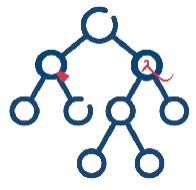
\includegraphics[height=1.0cm]{msca_logo.png}}%
    \end{center}

    \vspace{0.6cm}

    % Main title with Q logos on sides (with clickable links)
    \begin{center}
        \begin{minipage}{0.1\textwidth}
            \centering
            \href{https://quantlet.com}{
\includegraphics[height=1.1cm]{ql_logo.png}}
        \end{minipage}%
        \begin{minipage}{0.78\textwidth}
            \centering
            {\LARGE\bfseries\usebeamercolor[fg]{title}\inserttitle}

            \vspace{0.3cm}

            {\usebeamerfont{subtitle}\usebeamercolor[fg]{title}\insertsubtitle}
        \end{minipage}%
        \begin{minipage}{0.1\textwidth}
            \centering
            \href{https://quantinar.com}{
\includegraphics[height=1.1cm]{qr_logo.png}}
        \end{minipage}
    \end{center}

    \vspace{0.6cm}

    % Authors (left aligned)
    \hspace{0.5cm}{\usebeamerfont{author}\insertauthor}

    \vspace{0.3cm}

    % Institute/Affiliations (left aligned)
    \hspace{0.5cm}\begin{minipage}[t]{0.9\textwidth}
        \raggedright\small\insertinstitute
    \end{minipage}
}

%=============================================================================
% THEOREM ENVIRONMENTS
%=============================================================================
\theoremstyle{definition}
\setbeamertemplate{theorems}[numbered]
\ifdefined\tsalang
\newtheorem{defn}{Definiție}
\newtheorem{thm}{Teoremă}
\newtheorem{prop}{Propoziție}
\newtheorem{rmk}{Observație}
\else
\newtheorem{defn}{Definition}
\newtheorem{thm}{Theorem}
\newtheorem{prop}{Proposition}
\newtheorem{rmk}{Remark}
\fi

%=============================================================================
% CENTRED MINIPAGE (no extra vertical space)
%=============================================================================
\newenvironment{cminipage}[1]{%
    \par\noindent\hfill\begin{minipage}{#1}\ignorespaces
}{%
    \end{minipage}\hfill\null\par
}

%=============================================================================
% CUSTOM COMMANDS
%=============================================================================
\newcommand{\E}{\mathbb{E}}
\newcommand{\Var}{\text{Var}}
\newcommand{\Cov}{\text{Cov}}
\newcommand{\Corr}{\text{Corr}}
\newcommand{\R}{\mathbb{R}}
\newcommand{\N}{\mathbb{N}}
\newcommand{\Z}{\mathbb{Z}}
\newcommand{\B}{\mathbf{B}}
\newcommand{\imark}{\textcolor{MainBlue}{\textbullet}}
\newcommand{\RMSE}{\text{RMSE}}
\newcommand{\MAE}{\text{MAE}}
\newcommand{\MAPE}{\text{MAPE}}

% Boldface vector/matrix commands (VAR, VECM, state space; also used by the older TSA decks)
\newcommand{\bY}{\mathbf{Y}}
\newcommand{\bX}{\mathbf{X}}
\newcommand{\bA}{\mathbf{A}}
\newcommand{\bB}{\mathbf{B}}
\newcommand{\bepsilon}{\boldsymbol{\varepsilon}}
\newcommand{\bSigma}{\boldsymbol{\Sigma}}
\newcommand{\bPhi}{\boldsymbol{\Phi}}
\newcommand{\bGamma}{\boldsymbol{\Gamma}}
\newcommand{\bPi}{\boldsymbol{\Pi}}
\newcommand{\bc}{\mathbf{c}}
\newcommand{\balpha}{\boldsymbol{\alpha}}
\newcommand{\bbeta}{\boldsymbol{\beta}}
\newcommand{\bvarepsilon}{\boldsymbol{\varepsilon}}

% Legacy seminar marks (older TSA seminar decks)
\newcommand{\correct}{\textcolor{Forest}{\checkmark}}
\newcommand{\incorrect}{\textcolor{Crimson}{\texttimes}}
 se definește
%   \newcommand{\coursename}{Time Series Analysis}      (EN)
%   \newcommand{\coursename}{Serii de timp}       (RO)  și  \def\tsalang{ro}
% Fișierele .tex se află în EN/Courses, EN/Seminars, RO/Cursuri, RO/Seminarii (două niveluri sub rădăcină).
% Deck-urile sînt generate de latex/build_chapterN.py / build_seminarN.py (vezi latex/tsa_build.py).

\documentclass[9pt, aspectratio=169, t]{beamer}
\providecommand{\coursename}{Time Series Analysis}

% Ensure content fits on slides
\setbeamersize{text margin left=8mm, text margin right=8mm}
% Smaller institute font (title page)
\setbeamerfont{institute}{size=\footnotesize}

%=============================================================================
% THEME AND STYLE CONFIGURATION
%=============================================================================
\usetheme{default}
% Using default theme for clean header/footer control

% Color Palette (matching Redispatch PDF)
\definecolor{MainBlue}{RGB}{26, 58, 110}
\definecolor{AccentBlue}{RGB}{26, 58, 110}
\definecolor{IDAred}{RGB}{205, 0, 0}
\definecolor{DarkGray}{RGB}{51, 51, 51}
\definecolor{MediumGray}{RGB}{128, 128, 128}
\definecolor{LightGray}{RGB}{248, 248, 248}
\definecolor{VeryLightGray}{RGB}{235, 235, 235}
\definecolor{KeynoteGray}{RGB}{218, 218, 218}
\definecolor{SectionGray}{RGB}{120, 120, 120}
\definecolor{FooterGray}{RGB}{100, 100, 100}
\definecolor{Crimson}{RGB}{220, 53, 69}
\definecolor{Forest}{RGB}{46, 125, 50}
\definecolor{Amber}{RGB}{181, 133, 63}
\definecolor{Orange}{RGB}{230, 126, 34}
\definecolor{Purple}{RGB}{142, 68, 173}

% Gradient background (exact Keynote 315° gradient: white to RGB 218,218,218)
\setbeamertemplate{background}{%
    \begin{tikzpicture}[remember picture, overlay]
        \shade[shading=axis, shading angle=315,
        top color=white, bottom color=KeynoteGray]
        (current page.south west) rectangle (current page.north east);
    \end{tikzpicture}%
}
% Fallback solid color for compatibility
\setbeamercolor{background canvas}{bg=}

\setbeamercolor{palette primary}{bg=MainBlue, fg=white}
\setbeamercolor{palette secondary}{bg=MainBlue!85, fg=white}
\setbeamercolor{palette tertiary}{bg=MainBlue!70, fg=white}
\setbeamercolor{structure}{fg=MainBlue}
\setbeamercolor{title}{fg=IDAred}
\setbeamercolor{frametitle}{fg=IDAred, bg=}
\setbeamercolor{block title}{bg=MainBlue, fg=white}
\setbeamercolor{block body}{bg=VeryLightGray, fg=DarkGray}
\setbeamercolor{block title alerted}{bg=Crimson, fg=white}
\setbeamercolor{block body alerted}{bg=Crimson!8, fg=DarkGray}
\setbeamercolor{block title example}{bg=Forest, fg=white}
\setbeamercolor{block body example}{bg=Forest!8, fg=DarkGray}
\setbeamercolor{item}{fg=MainBlue}

% Footer colors (override Madrid theme blue)
\setbeamercolor{author in head/foot}{fg=FooterGray, bg=}
\setbeamercolor{title in head/foot}{fg=FooterGray, bg=}
\setbeamercolor{date in head/foot}{fg=FooterGray, bg=}
\setbeamercolor{section in head/foot}{fg=FooterGray, bg=}
\setbeamercolor{subsection in head/foot}{fg=FooterGray, bg=}

% Bullet styles (apply everywhere including blocks)
\setbeamertemplate{itemize item}{\color{MainBlue}$\boxdot$}
\setbeamertemplate{itemize subitem}{\color{MainBlue}$\blacktriangleright$}
\setbeamertemplate{itemize subsubitem}{\color{MainBlue}\tiny$\bullet$}
\setbeamertemplate{itemize/enumerate body begin}{\normalsize}
\setbeamertemplate{itemize/enumerate subbody begin}{\normalsize}

% Item spacing - compact style
\setlength{\leftmargini}{10pt}       % Level 1: minimal indent
\setlength{\leftmarginii}{10pt}      % Level 2: minimal additional indent
% Compact list spacing (zero extra space before/after lists in blocks)
\makeatletter
\def\@listi{\leftmargin\leftmargini \topsep 0pt \parsep 0pt \itemsep 0pt}
\def\@listii{\leftmargin\leftmarginii \topsep 0pt \parsep 0pt \itemsep 0pt}
\makeatother

\setbeamertemplate{navigation symbols}{}

%=============================================================================
% CUSTOM HEADLINE
%=============================================================================
\setbeamertemplate{headline}{%
    \vskip10pt%
    \hbox to \paperwidth{%
        \hskip0.5cm%
        {\small\color{FooterGray}\renewcommand{\hyperlink}[2]{##2}\insertsectionhead}%
        \hfill%
        \textcolor{FooterGray}{\small\insertframenumber}%
        \hskip0.5cm%
    }%
    \vskip4pt%
    {\color{FooterGray}\hrule height 0.4pt}%
}

%=============================================================================
% CUSTOM FOOTER
%=============================================================================
\usepackage{fontawesome5}

\setbeamertemplate{footline}{%
    {\color{FooterGray}\hrule height 0.4pt}%
    \vskip4pt%
    \hbox to \paperwidth{%
        \hskip0.5cm%
        \textcolor{FooterGray}{\small\coursename}%
        \hfill%
        \raisebox{-0.1em}{%
            \begin{tikzpicture}[x=0.08em, y=0.08em, line width=0.4pt]
                \draw[FooterGray] (0,3) -- (1,4) -- (2,3.5) -- (3,5) -- (4,4) -- (5,6) -- (6,5.5) -- (7,4) -- (8,5) -- (9,7) -- (10,6) -- (11,5) -- (12,6.5) -- (13,8) -- (14,7) -- (15,6) -- (16,7.5) -- (17,9) -- (18,8) -- (19,7) -- (20,8.5) -- (21,10) -- (22,9) -- (23,8) -- (24,9.5);
            \end{tikzpicture}%
        }%
        \hskip0.5cm%
    }%
    \vskip6pt%
}

%=============================================================================
% PACKAGES
%=============================================================================
\usepackage[utf8]{inputenc}
\DeclareUnicodeCharacter{03B1}{\ensuremath{\alpha}}
\usepackage[T1]{fontenc}
\usepackage{amsmath, amssymb, amsthm}
\usepackage{mathtools}
\usepackage{bm}
\usepackage{tikz}
\usetikzlibrary{arrows.meta, positioning, shapes, calc, decorations.pathreplacing, shadings}
\usepackage{booktabs}
\usepackage{multirow}
\usepackage{array}
\usepackage{graphicx}
\usepackage{animate}
\usepackage{hyperref}
\usepackage{colortbl}
\usepackage{listings}
\lstset{language=Python, basicstyle=\ttfamily\scriptsize, keywordstyle=\color{MainBlue}\bfseries,
  commentstyle=\color{Forest}, stringstyle=\color{Crimson}, breaklines=true,
  frame=none, backgroundcolor=\color{VeryLightGray}, xleftmargin=2mm}
\hypersetup{colorlinks=true, linkcolor=MainBlue, urlcolor=MainBlue}
\graphicspath{{../../logos/}{../../charts/}{../../photos/}}
\usepackage{xcolor}
\hfuzz=2pt  % Suppress tiny overfull warnings (<2pt)
\vfuzz=2pt  % Suppress tiny vertical overfull warnings (<2pt)
% \mathrm in the sans-serif family of the slides (beamer resets \mathrm to the serif family at \begin{document};
% this hook runs after beamer's, so WN, Var, RMSE, ... in formulas match the surrounding text)
% Bold vectors and matrices in the same sans-serif family: \mathbf{A} in sans bold (beamer's own \mathbf came out in
% medium weight), and the bold upright Greek capitals of \boldsymbol / \bm (\bSigma, \bPhi, \boldsymbol{\Theta}) in
% cmss bold: bm.sty fixes its "boldoperators" font when it is loaded (serif cmbx), before beamer switches the
% operators to cmss, so it is reset here.
\AtBeginDocument{%
  \SetMathAlphabet{\mathrm}{normal}{\encodingdefault}{\sfdefault}{\mddefault}{n}%
  \SetMathAlphabet{\mathrm}{bold}{\encodingdefault}{\sfdefault}{bx}{n}%
  \SetMathAlphabet{\mathbf}{normal}{\encodingdefault}{\sfdefault}{bx}{n}%
  \SetMathAlphabet{\mathbf}{bold}{\encodingdefault}{\sfdefault}{bx}{n}%
  \SetSymbolFont{boldoperators}{normal}{OT1}{cmss}{bx}{n}%
  \SetSymbolFont{boldoperators}{bold}{OT1}{cmss}{bx}{n}}

%=============================================================================
% QUANTLET COMMANDS
%   \quantlet{<displayed name>}{<url>}       (generic, compatible with the older TSA decks)
%   \tsaquantlet{Ch_05}{TSA_ch5_garch}       -> https://github.com/danpele/Time-Series-Analysis/tree/main/Quantlets/Ch_05/TSA_ch5_garch
%   \qlurl{<folder>} is defined per chapter by the generator (Quantlets/Ch_NN/<folder>)
%=============================================================================
\newcommand{\tsarepo}{https://github.com/danpele/Time-Series-Analysis}
\newcommand{\tsaqlbase}{https://github.com/danpele/Time-Series-Analysis/tree/main/Quantlets}
\newcommand{\quantlet}[2]{%
    \hfill\href{#2}{%
        \raisebox{-0.15em}{
\includegraphics[height=0.7em]{ql_logo.png}}%
        \textcolor{MainBlue}{\tiny\ #1}%
    }%
}
\newcommand{\tsaquantlet}[2]{\quantlet{\detokenize{#2}}{\tsaqlbase/#1/#2}}

%=============================================================================
% NOTEBOOKS (Google Colab)
%   \colaburl{notebooks/EN/chapter5_seminar_notebook.ipynb} -> the Colab link of a file in the TSA repo
%   \nb: the chapter notebook (each seminar deck redefines it with \renewcommand)
%=============================================================================
\newcommand{\colaburl}[1]{https://colab.research.google.com/github/danpele/Time-Series-Analysis/blob/main/#1}
\newcommand{\nb}{https://colab.research.google.com/github/danpele/Time-Series-Analysis/tree/main/notebooks/EN}
\newcommand{\nbname}{notebooks/EN}

%=============================================================================
% SLIDE HELPERS (used by the generators; the same as in MFM)
%=============================================================================
% local font size for list bodies (the preamble forces \normalsize)
\newcommand{\itemsize}[1]{\setbeamertemplate{itemize/enumerate body begin}{#1}\setbeamertemplate{itemize/enumerate subbody begin}{#1}}
\newcommand{\intitle}[1]{{\hypersetup{urlcolor=white}#1}}   % white links inside coloured title bars
\newcommand{\imgcap}[1]{{\scriptsize #1}\\[0.5mm]}          % caption under a photo
\newcommand{\imgcredit}[2]{{\tiny\color{FooterGray}\href{#1}{#2}}}   % image credit: source URL, author/licence
\newcommand{\aiprompt}[1]{{\ttfamily\color{MainBlue}#1}}     % a prompt to an AI assistant

%=============================================================================
% SEMINARS: student version by default; the instructor wrapper *_solutions.tex sets \solutionstrue
%=============================================================================
\makeatletter\@ifundefined{ifsolutions}{\expandafter\newif\csname ifsolutions\endcsname}{}\makeatother
\newcommand{\solonly}[1]{\ifsolutions #1\fi}
\newcommand{\propsub}{\ifsolutions\else\framesubtitle{\ifdefined\tsalang Rezolvarea se discută la seminar\else Solution discussed in class\fi}\fi}

%=============================================================================
% APPENDIX AND CHAPTER LINKS (latex/appendix_links.py writes the calls; it also re-declares these
% macros before \begin{document}, so the decks compile with or without this preamble block)
%=============================================================================
\providecommand{\tsaapplink}[3]{\hypertarget{#2}{}\hyperlink{#1}{\beamergotobutton{#3}}}
\providecommand{\tsaappback}[2]{\begin{tikzpicture}[remember picture,overlay]\node[anchor=south east] at ([xshift=-3mm,yshift=7mm]current page.south east){\hyperlink{#1}{\beamerreturnbutton{#2}}};\end{tikzpicture}}
\providecommand{\tsachlink}[2]{\href{#1}{#2}}
\providecommand{\tsachlinkt}[2]{\href{#1}{\usebeamercolor[fg]{frametitle}#2}}

%=============================================================================
% QUANTINAR COMMAND: link către un curs Quantinar (subiecte avansate)
%=============================================================================
\newcommand{\quantinar}[2]{%
    \href{#2}{%
        \raisebox{-0.15em}{
\includegraphics[height=0.8em]{qr_logo.png}}%
        \textcolor{MainBlue}{\scriptsize\ #1}%
    }%
}

%=============================================================================
% CUSTOM TITLE PAGE
%=============================================================================
\defbeamertemplate*{title page}{hybrid}[1][]
{
    \vspace{0.2cm}
    % Logos row - top header (with clickable links)
    \begin{center}
        \href{https://www.ase.ro}{
\includegraphics[height=1.0cm]{ase_logo.png}}\hspace{0.3cm}%
        \href{https://theida.net}{
\includegraphics[height=1.0cm]{ida_logo.png}}\hspace{0.3cm}%
        \href{https://blockchain-research-center.com}{
\includegraphics[height=1.0cm]{brc_logo.png}}\hspace{0.3cm}%
        \href{https://www.ai4efin.ase.ro}{
\includegraphics[height=1.0cm]{ai4efin_logo.png}}\hspace{0.3cm}%
        \href{https://ipe.ro/new}{
\includegraphics[height=1.0cm]{acad_logo.png}}\hspace{0.3cm}%
        \href{https://www.digital-finance-msca.com}{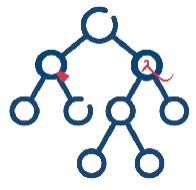
\includegraphics[height=1.0cm]{msca_logo.png}}%
    \end{center}

    \vspace{0.6cm}

    % Main title with Q logos on sides (with clickable links)
    \begin{center}
        \begin{minipage}{0.1\textwidth}
            \centering
            \href{https://quantlet.com}{
\includegraphics[height=1.1cm]{ql_logo.png}}
        \end{minipage}%
        \begin{minipage}{0.78\textwidth}
            \centering
            {\LARGE\bfseries\usebeamercolor[fg]{title}\inserttitle}

            \vspace{0.3cm}

            {\usebeamerfont{subtitle}\usebeamercolor[fg]{title}\insertsubtitle}
        \end{minipage}%
        \begin{minipage}{0.1\textwidth}
            \centering
            \href{https://quantinar.com}{
\includegraphics[height=1.1cm]{qr_logo.png}}
        \end{minipage}
    \end{center}

    \vspace{0.6cm}

    % Authors (left aligned)
    \hspace{0.5cm}{\usebeamerfont{author}\insertauthor}

    \vspace{0.3cm}

    % Institute/Affiliations (left aligned)
    \hspace{0.5cm}\begin{minipage}[t]{0.9\textwidth}
        \raggedright\small\insertinstitute
    \end{minipage}
}

%=============================================================================
% THEOREM ENVIRONMENTS
%=============================================================================
\theoremstyle{definition}
\setbeamertemplate{theorems}[numbered]
\ifdefined\tsalang
\newtheorem{defn}{Definiție}
\newtheorem{thm}{Teoremă}
\newtheorem{prop}{Propoziție}
\newtheorem{rmk}{Observație}
\else
\newtheorem{defn}{Definition}
\newtheorem{thm}{Theorem}
\newtheorem{prop}{Proposition}
\newtheorem{rmk}{Remark}
\fi

%=============================================================================
% CENTRED MINIPAGE (no extra vertical space)
%=============================================================================
\newenvironment{cminipage}[1]{%
    \par\noindent\hfill\begin{minipage}{#1}\ignorespaces
}{%
    \end{minipage}\hfill\null\par
}

%=============================================================================
% CUSTOM COMMANDS
%=============================================================================
\newcommand{\E}{\mathbb{E}}
\newcommand{\Var}{\text{Var}}
\newcommand{\Cov}{\text{Cov}}
\newcommand{\Corr}{\text{Corr}}
\newcommand{\R}{\mathbb{R}}
\newcommand{\N}{\mathbb{N}}
\newcommand{\Z}{\mathbb{Z}}
\newcommand{\B}{\mathbf{B}}
\newcommand{\imark}{\textcolor{MainBlue}{\textbullet}}
\newcommand{\RMSE}{\text{RMSE}}
\newcommand{\MAE}{\text{MAE}}
\newcommand{\MAPE}{\text{MAPE}}

% Boldface vector/matrix commands (VAR, VECM, state space; also used by the older TSA decks)
\newcommand{\bY}{\mathbf{Y}}
\newcommand{\bX}{\mathbf{X}}
\newcommand{\bA}{\mathbf{A}}
\newcommand{\bB}{\mathbf{B}}
\newcommand{\bepsilon}{\boldsymbol{\varepsilon}}
\newcommand{\bSigma}{\boldsymbol{\Sigma}}
\newcommand{\bPhi}{\boldsymbol{\Phi}}
\newcommand{\bGamma}{\boldsymbol{\Gamma}}
\newcommand{\bPi}{\boldsymbol{\Pi}}
\newcommand{\bc}{\mathbf{c}}
\newcommand{\balpha}{\boldsymbol{\alpha}}
\newcommand{\bbeta}{\boldsymbol{\beta}}
\newcommand{\bvarepsilon}{\boldsymbol{\varepsilon}}

% Legacy seminar marks (older TSA seminar decks)
\newcommand{\correct}{\textcolor{Forest}{\checkmark}}
\newcommand{\incorrect}{\textcolor{Crimson}{\texttimes}}
 se definește
%   \newcommand{\coursename}{Time Series Analysis}      (EN)
%   \newcommand{\coursename}{Serii de timp}       (RO)  și  \def\tsalang{ro}
% Fișierele .tex se află în EN/Courses, EN/Seminars, RO/Cursuri, RO/Seminarii (două niveluri sub rădăcină).
% Deck-urile sînt generate de latex/build_chapterN.py / build_seminarN.py (vezi latex/tsa_build.py).

\documentclass[9pt, aspectratio=169, t]{beamer}
\providecommand{\coursename}{Time Series Analysis}

% Ensure content fits on slides
\setbeamersize{text margin left=8mm, text margin right=8mm}
% Smaller institute font (title page)
\setbeamerfont{institute}{size=\footnotesize}

%=============================================================================
% THEME AND STYLE CONFIGURATION
%=============================================================================
\usetheme{default}
% Using default theme for clean header/footer control

% Color Palette (matching Redispatch PDF)
\definecolor{MainBlue}{RGB}{26, 58, 110}
\definecolor{AccentBlue}{RGB}{26, 58, 110}
\definecolor{IDAred}{RGB}{205, 0, 0}
\definecolor{DarkGray}{RGB}{51, 51, 51}
\definecolor{MediumGray}{RGB}{128, 128, 128}
\definecolor{LightGray}{RGB}{248, 248, 248}
\definecolor{VeryLightGray}{RGB}{235, 235, 235}
\definecolor{KeynoteGray}{RGB}{218, 218, 218}
\definecolor{SectionGray}{RGB}{120, 120, 120}
\definecolor{FooterGray}{RGB}{100, 100, 100}
\definecolor{Crimson}{RGB}{220, 53, 69}
\definecolor{Forest}{RGB}{46, 125, 50}
\definecolor{Amber}{RGB}{181, 133, 63}
\definecolor{Orange}{RGB}{230, 126, 34}
\definecolor{Purple}{RGB}{142, 68, 173}

% Gradient background (exact Keynote 315° gradient: white to RGB 218,218,218)
\setbeamertemplate{background}{%
    \begin{tikzpicture}[remember picture, overlay]
        \shade[shading=axis, shading angle=315,
        top color=white, bottom color=KeynoteGray]
        (current page.south west) rectangle (current page.north east);
    \end{tikzpicture}%
}
% Fallback solid color for compatibility
\setbeamercolor{background canvas}{bg=}

\setbeamercolor{palette primary}{bg=MainBlue, fg=white}
\setbeamercolor{palette secondary}{bg=MainBlue!85, fg=white}
\setbeamercolor{palette tertiary}{bg=MainBlue!70, fg=white}
\setbeamercolor{structure}{fg=MainBlue}
\setbeamercolor{title}{fg=IDAred}
\setbeamercolor{frametitle}{fg=IDAred, bg=}
\setbeamercolor{block title}{bg=MainBlue, fg=white}
\setbeamercolor{block body}{bg=VeryLightGray, fg=DarkGray}
\setbeamercolor{block title alerted}{bg=Crimson, fg=white}
\setbeamercolor{block body alerted}{bg=Crimson!8, fg=DarkGray}
\setbeamercolor{block title example}{bg=Forest, fg=white}
\setbeamercolor{block body example}{bg=Forest!8, fg=DarkGray}
\setbeamercolor{item}{fg=MainBlue}

% Footer colors (override Madrid theme blue)
\setbeamercolor{author in head/foot}{fg=FooterGray, bg=}
\setbeamercolor{title in head/foot}{fg=FooterGray, bg=}
\setbeamercolor{date in head/foot}{fg=FooterGray, bg=}
\setbeamercolor{section in head/foot}{fg=FooterGray, bg=}
\setbeamercolor{subsection in head/foot}{fg=FooterGray, bg=}

% Bullet styles (apply everywhere including blocks)
\setbeamertemplate{itemize item}{\color{MainBlue}$\boxdot$}
\setbeamertemplate{itemize subitem}{\color{MainBlue}$\blacktriangleright$}
\setbeamertemplate{itemize subsubitem}{\color{MainBlue}\tiny$\bullet$}
\setbeamertemplate{itemize/enumerate body begin}{\normalsize}
\setbeamertemplate{itemize/enumerate subbody begin}{\normalsize}

% Item spacing - compact style
\setlength{\leftmargini}{10pt}       % Level 1: minimal indent
\setlength{\leftmarginii}{10pt}      % Level 2: minimal additional indent
% Compact list spacing (zero extra space before/after lists in blocks)
\makeatletter
\def\@listi{\leftmargin\leftmargini \topsep 0pt \parsep 0pt \itemsep 0pt}
\def\@listii{\leftmargin\leftmarginii \topsep 0pt \parsep 0pt \itemsep 0pt}
\makeatother

\setbeamertemplate{navigation symbols}{}

%=============================================================================
% CUSTOM HEADLINE
%=============================================================================
\setbeamertemplate{headline}{%
    \vskip10pt%
    \hbox to \paperwidth{%
        \hskip0.5cm%
        {\small\color{FooterGray}\renewcommand{\hyperlink}[2]{##2}\insertsectionhead}%
        \hfill%
        \textcolor{FooterGray}{\small\insertframenumber}%
        \hskip0.5cm%
    }%
    \vskip4pt%
    {\color{FooterGray}\hrule height 0.4pt}%
}

%=============================================================================
% CUSTOM FOOTER
%=============================================================================
\usepackage{fontawesome5}

\setbeamertemplate{footline}{%
    {\color{FooterGray}\hrule height 0.4pt}%
    \vskip4pt%
    \hbox to \paperwidth{%
        \hskip0.5cm%
        \textcolor{FooterGray}{\small\coursename}%
        \hfill%
        \raisebox{-0.1em}{%
            \begin{tikzpicture}[x=0.08em, y=0.08em, line width=0.4pt]
                \draw[FooterGray] (0,3) -- (1,4) -- (2,3.5) -- (3,5) -- (4,4) -- (5,6) -- (6,5.5) -- (7,4) -- (8,5) -- (9,7) -- (10,6) -- (11,5) -- (12,6.5) -- (13,8) -- (14,7) -- (15,6) -- (16,7.5) -- (17,9) -- (18,8) -- (19,7) -- (20,8.5) -- (21,10) -- (22,9) -- (23,8) -- (24,9.5);
            \end{tikzpicture}%
        }%
        \hskip0.5cm%
    }%
    \vskip6pt%
}

%=============================================================================
% PACKAGES
%=============================================================================
\usepackage[utf8]{inputenc}
\DeclareUnicodeCharacter{03B1}{\ensuremath{\alpha}}
\usepackage[T1]{fontenc}
\usepackage{amsmath, amssymb, amsthm}
\usepackage{mathtools}
\usepackage{bm}
\usepackage{tikz}
\usetikzlibrary{arrows.meta, positioning, shapes, calc, decorations.pathreplacing, shadings}
\usepackage{booktabs}
\usepackage{multirow}
\usepackage{array}
\usepackage{graphicx}
\usepackage{animate}
\usepackage{hyperref}
\usepackage{colortbl}
\usepackage{listings}
\lstset{language=Python, basicstyle=\ttfamily\scriptsize, keywordstyle=\color{MainBlue}\bfseries,
  commentstyle=\color{Forest}, stringstyle=\color{Crimson}, breaklines=true,
  frame=none, backgroundcolor=\color{VeryLightGray}, xleftmargin=2mm}
\hypersetup{colorlinks=true, linkcolor=MainBlue, urlcolor=MainBlue}
\graphicspath{{../../logos/}{../../charts/}{../../photos/}}
\usepackage{xcolor}
\hfuzz=2pt  % Suppress tiny overfull warnings (<2pt)
\vfuzz=2pt  % Suppress tiny vertical overfull warnings (<2pt)
% \mathrm in the sans-serif family of the slides (beamer resets \mathrm to the serif family at \begin{document};
% this hook runs after beamer's, so WN, Var, RMSE, ... in formulas match the surrounding text)
% Bold vectors and matrices in the same sans-serif family: \mathbf{A} in sans bold (beamer's own \mathbf came out in
% medium weight), and the bold upright Greek capitals of \boldsymbol / \bm (\bSigma, \bPhi, \boldsymbol{\Theta}) in
% cmss bold: bm.sty fixes its "boldoperators" font when it is loaded (serif cmbx), before beamer switches the
% operators to cmss, so it is reset here.
\AtBeginDocument{%
  \SetMathAlphabet{\mathrm}{normal}{\encodingdefault}{\sfdefault}{\mddefault}{n}%
  \SetMathAlphabet{\mathrm}{bold}{\encodingdefault}{\sfdefault}{bx}{n}%
  \SetMathAlphabet{\mathbf}{normal}{\encodingdefault}{\sfdefault}{bx}{n}%
  \SetMathAlphabet{\mathbf}{bold}{\encodingdefault}{\sfdefault}{bx}{n}%
  \SetSymbolFont{boldoperators}{normal}{OT1}{cmss}{bx}{n}%
  \SetSymbolFont{boldoperators}{bold}{OT1}{cmss}{bx}{n}}

%=============================================================================
% QUANTLET COMMANDS
%   \quantlet{<displayed name>}{<url>}       (generic, compatible with the older TSA decks)
%   \tsaquantlet{Ch_05}{TSA_ch5_garch}       -> https://github.com/danpele/Time-Series-Analysis/tree/main/Quantlets/Ch_05/TSA_ch5_garch
%   \qlurl{<folder>} is defined per chapter by the generator (Quantlets/Ch_NN/<folder>)
%=============================================================================
\newcommand{\tsarepo}{https://github.com/danpele/Time-Series-Analysis}
\newcommand{\tsaqlbase}{https://github.com/danpele/Time-Series-Analysis/tree/main/Quantlets}
\newcommand{\quantlet}[2]{%
    \hfill\href{#2}{%
        \raisebox{-0.15em}{
\includegraphics[height=0.7em]{ql_logo.png}}%
        \textcolor{MainBlue}{\tiny\ #1}%
    }%
}
\newcommand{\tsaquantlet}[2]{\quantlet{\detokenize{#2}}{\tsaqlbase/#1/#2}}

%=============================================================================
% NOTEBOOKS (Google Colab)
%   \colaburl{notebooks/EN/chapter5_seminar_notebook.ipynb} -> the Colab link of a file in the TSA repo
%   \nb: the chapter notebook (each seminar deck redefines it with \renewcommand)
%=============================================================================
\newcommand{\colaburl}[1]{https://colab.research.google.com/github/danpele/Time-Series-Analysis/blob/main/#1}
\newcommand{\nb}{https://colab.research.google.com/github/danpele/Time-Series-Analysis/tree/main/notebooks/EN}
\newcommand{\nbname}{notebooks/EN}

%=============================================================================
% SLIDE HELPERS (used by the generators; the same as in MFM)
%=============================================================================
% local font size for list bodies (the preamble forces \normalsize)
\newcommand{\itemsize}[1]{\setbeamertemplate{itemize/enumerate body begin}{#1}\setbeamertemplate{itemize/enumerate subbody begin}{#1}}
\newcommand{\intitle}[1]{{\hypersetup{urlcolor=white}#1}}   % white links inside coloured title bars
\newcommand{\imgcap}[1]{{\scriptsize #1}\\[0.5mm]}          % caption under a photo
\newcommand{\imgcredit}[2]{{\tiny\color{FooterGray}\href{#1}{#2}}}   % image credit: source URL, author/licence
\newcommand{\aiprompt}[1]{{\ttfamily\color{MainBlue}#1}}     % a prompt to an AI assistant

%=============================================================================
% SEMINARS: student version by default; the instructor wrapper *_solutions.tex sets \solutionstrue
%=============================================================================
\makeatletter\@ifundefined{ifsolutions}{\expandafter\newif\csname ifsolutions\endcsname}{}\makeatother
\newcommand{\solonly}[1]{\ifsolutions #1\fi}
\newcommand{\propsub}{\ifsolutions\else\framesubtitle{\ifdefined\tsalang Rezolvarea se discută la seminar\else Solution discussed in class\fi}\fi}

%=============================================================================
% APPENDIX AND CHAPTER LINKS (latex/appendix_links.py writes the calls; it also re-declares these
% macros before \begin{document}, so the decks compile with or without this preamble block)
%=============================================================================
\providecommand{\tsaapplink}[3]{\hypertarget{#2}{}\hyperlink{#1}{\beamergotobutton{#3}}}
\providecommand{\tsaappback}[2]{\begin{tikzpicture}[remember picture,overlay]\node[anchor=south east] at ([xshift=-3mm,yshift=7mm]current page.south east){\hyperlink{#1}{\beamerreturnbutton{#2}}};\end{tikzpicture}}
\providecommand{\tsachlink}[2]{\href{#1}{#2}}
\providecommand{\tsachlinkt}[2]{\href{#1}{\usebeamercolor[fg]{frametitle}#2}}

%=============================================================================
% QUANTINAR COMMAND: link către un curs Quantinar (subiecte avansate)
%=============================================================================
\newcommand{\quantinar}[2]{%
    \href{#2}{%
        \raisebox{-0.15em}{
\includegraphics[height=0.8em]{qr_logo.png}}%
        \textcolor{MainBlue}{\scriptsize\ #1}%
    }%
}

%=============================================================================
% CUSTOM TITLE PAGE
%=============================================================================
\defbeamertemplate*{title page}{hybrid}[1][]
{
    \vspace{0.2cm}
    % Logos row - top header (with clickable links)
    \begin{center}
        \href{https://www.ase.ro}{
\includegraphics[height=1.0cm]{ase_logo.png}}\hspace{0.3cm}%
        \href{https://theida.net}{
\includegraphics[height=1.0cm]{ida_logo.png}}\hspace{0.3cm}%
        \href{https://blockchain-research-center.com}{
\includegraphics[height=1.0cm]{brc_logo.png}}\hspace{0.3cm}%
        \href{https://www.ai4efin.ase.ro}{
\includegraphics[height=1.0cm]{ai4efin_logo.png}}\hspace{0.3cm}%
        \href{https://ipe.ro/new}{
\includegraphics[height=1.0cm]{acad_logo.png}}\hspace{0.3cm}%
        \href{https://www.digital-finance-msca.com}{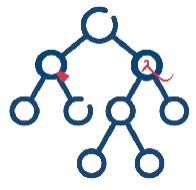
\includegraphics[height=1.0cm]{msca_logo.png}}%
    \end{center}

    \vspace{0.6cm}

    % Main title with Q logos on sides (with clickable links)
    \begin{center}
        \begin{minipage}{0.1\textwidth}
            \centering
            \href{https://quantlet.com}{
\includegraphics[height=1.1cm]{ql_logo.png}}
        \end{minipage}%
        \begin{minipage}{0.78\textwidth}
            \centering
            {\LARGE\bfseries\usebeamercolor[fg]{title}\inserttitle}

            \vspace{0.3cm}

            {\usebeamerfont{subtitle}\usebeamercolor[fg]{title}\insertsubtitle}
        \end{minipage}%
        \begin{minipage}{0.1\textwidth}
            \centering
            \href{https://quantinar.com}{
\includegraphics[height=1.1cm]{qr_logo.png}}
        \end{minipage}
    \end{center}

    \vspace{0.6cm}

    % Authors (left aligned)
    \hspace{0.5cm}{\usebeamerfont{author}\insertauthor}

    \vspace{0.3cm}

    % Institute/Affiliations (left aligned)
    \hspace{0.5cm}\begin{minipage}[t]{0.9\textwidth}
        \raggedright\small\insertinstitute
    \end{minipage}
}

%=============================================================================
% THEOREM ENVIRONMENTS
%=============================================================================
\theoremstyle{definition}
\setbeamertemplate{theorems}[numbered]
\ifdefined\tsalang
\newtheorem{defn}{Definiție}
\newtheorem{thm}{Teoremă}
\newtheorem{prop}{Propoziție}
\newtheorem{rmk}{Observație}
\else
\newtheorem{defn}{Definition}
\newtheorem{thm}{Theorem}
\newtheorem{prop}{Proposition}
\newtheorem{rmk}{Remark}
\fi

%=============================================================================
% CENTRED MINIPAGE (no extra vertical space)
%=============================================================================
\newenvironment{cminipage}[1]{%
    \par\noindent\hfill\begin{minipage}{#1}\ignorespaces
}{%
    \end{minipage}\hfill\null\par
}

%=============================================================================
% CUSTOM COMMANDS
%=============================================================================
\newcommand{\E}{\mathbb{E}}
\newcommand{\Var}{\text{Var}}
\newcommand{\Cov}{\text{Cov}}
\newcommand{\Corr}{\text{Corr}}
\newcommand{\R}{\mathbb{R}}
\newcommand{\N}{\mathbb{N}}
\newcommand{\Z}{\mathbb{Z}}
\newcommand{\B}{\mathbf{B}}
\newcommand{\imark}{\textcolor{MainBlue}{\textbullet}}
\newcommand{\RMSE}{\text{RMSE}}
\newcommand{\MAE}{\text{MAE}}
\newcommand{\MAPE}{\text{MAPE}}

% Boldface vector/matrix commands (VAR, VECM, state space; also used by the older TSA decks)
\newcommand{\bY}{\mathbf{Y}}
\newcommand{\bX}{\mathbf{X}}
\newcommand{\bA}{\mathbf{A}}
\newcommand{\bB}{\mathbf{B}}
\newcommand{\bepsilon}{\boldsymbol{\varepsilon}}
\newcommand{\bSigma}{\boldsymbol{\Sigma}}
\newcommand{\bPhi}{\boldsymbol{\Phi}}
\newcommand{\bGamma}{\boldsymbol{\Gamma}}
\newcommand{\bPi}{\boldsymbol{\Pi}}
\newcommand{\bc}{\mathbf{c}}
\newcommand{\balpha}{\boldsymbol{\alpha}}
\newcommand{\bbeta}{\boldsymbol{\beta}}
\newcommand{\bvarepsilon}{\boldsymbol{\varepsilon}}

% Legacy seminar marks (older TSA seminar decks)
\newcommand{\correct}{\textcolor{Forest}{\checkmark}}
\newcommand{\incorrect}{\textcolor{Crimson}{\texttimes}}


\newcommand{\qlurl}[1]{https://github.com/danpele/Time-Series-Analysis/tree/main/Quantlets/Ch_08/#1}
\renewcommand{\nb}{\colaburl{notebooks/EN/chapter8_seminar_notebook.ipynb}}
\renewcommand{\nbname}{chapter8\_seminar\_notebook.ipynb}
% left column: full width in the student version, narrower next to the solution
\newcommand{\taskw}{\ifsolutions 0.47\textwidth\else 0.96\textwidth\fi}
\newcommand{\solw}{\ifsolutions 0.49\textwidth\else 0pt\fi}

% Clickable citations (DOIs verified via Crossref)
\newcommand{\refHP}{\href{https://doi.org/10.1007/978-3-031-13584-2}{Huang și Petukhina (2022)}}
\newcommand{\refBDtm}{\href{https://doi.org/10.1007/978-1-4419-0320-4}{Brockwell și Davis (1991)}}
\newcommand{\refBeran}{\href{https://doi.org/10.1007/978-3-642-35512-7}{Beran et al.\ (2013)}}
\newcommand{\refBaillie}{\href{https://doi.org/10.1016/0304-4076(95)01732-1}{Baillie (1996)}}
\newcommand{\refGraves}{\href{https://doi.org/10.3390/e19090437}{Graves et al.\ (2017)}}
\newcommand{\refHurst}{\href{https://doi.org/10.1061/TACEAT.0006518}{Hurst (1951)}}
\newcommand{\refMVN}{\href{https://doi.org/10.1137/1010093}{Mandelbrot și Van Ness (1968)}}
\newcommand{\refNoah}{\href{https://doi.org/10.1029/WR004i005p00909}{Mandelbrot și Wallis (1968)}}
\newcommand{\refMW}{\href{https://doi.org/10.1029/WR005i005p00967}{Mandelbrot și Wallis (1969)}}
\newcommand{\refGJ}{\href{https://doi.org/10.1111/j.1467-9892.1980.tb00297.x}{Granger și Joyeux (1980)}}
\newcommand{\refHosking}{\href{https://doi.org/10.1093/biomet/68.1.165}{Hosking (1981)}}
\newcommand{\refLo}{\href{https://doi.org/10.2307/2938368}{Lo (1991)}}
\newcommand{\refPeng}{\href{https://doi.org/10.1103/PhysRevE.49.1685}{Peng et al.\ (1994)}}
\newcommand{\refGPH}{\href{https://doi.org/10.1111/j.1467-9892.1983.tb00371.x}{Geweke și Porter-Hudak (1983)}}
\newcommand{\refRob}{\href{https://doi.org/10.1214/aos/1176324317}{Robinson (1995)}}
\newcommand{\refVelasco}{\href{https://doi.org/10.1111/1467-9892.00127}{Velasco (1999)}}
\newcommand{\refSowell}{\href{https://doi.org/10.1016/0304-4076(92)90084-5}{Sowell (1992)}}
\newcommand{\refFT}{\href{https://doi.org/10.1214/aos/1176349936}{Fox și Taqqu (1986)}}
\newcommand{\refRay}{\href{https://doi.org/10.1111/j.1467-9892.1993.tb00161.x}{Ray (1993)}}
\newcommand{\refHW}{\href{https://doi.org/10.1080/07350015.1995.10524577}{Hassler și Wolters (1995)}}
\newcommand{\refDGE}{\href{https://doi.org/10.1016/0927-5398(93)90006-D}{Ding, Granger și Engle (1993)}}
\newcommand{\refBBM}{\href{https://doi.org/10.1016/S0304-4076(95)01749-6}{Baillie, Bollerslev și Mikkelsen (1996)}}
\newcommand{\refABDL}{\href{https://doi.org/10.1111/1468-0262.00418}{Andersen et al.\ (2003)}}
\newcommand{\refCorsi}{\href{https://doi.org/10.1093/jjfinec/nbp001}{Corsi (2009)}}
\newcommand{\refDI}{\href{https://doi.org/10.1016/S0304-4076(01)00073-2}{Diebold și Inoue (2001)}}
\newcommand{\refGH}{\href{https://doi.org/10.1016/j.jempfin.2003.03.001}{Granger și Hyung (2004)}}
\newcommand{\refCobb}{\href{https://doi.org/10.1093/biomet/65.2.243}{Cobb (1978)}}
\newcommand{\refWeron}{\href{https://doi.org/10.1016/S0378-4371(02)00961-5}{Weron (2002)}}
\newcommand{\refCL}{\href{https://doi.org/10.1080/07350015.1993.10509936}{Cheung și Lai (1993)}}

\title[Serii de timp]{Serii de timp}
\subtitle{Seminarul 8: Memorie lungă și ARFIMA\ifsolutions\ (versiunea profesorului)\fi}
\author[D.T. Pele]{Daniel Traian PELE}
\institute{Academia de Studii Economice din București\\
IDA Institute Digital Assets\\
Blockchain Research Center\\
AI4EFin Artificial Intelligence for Energy Finance\\
Academia Română, Institutul de Prognoză Economică\\
MSCA Digital Finance}
\date{}

%=============================================================================
\providecommand{\tsaapplink}[3]{\hypertarget{#2}{}\hyperlink{#1}{\beamergotobutton{#3}}}  % APPLINKS-MACROS
\providecommand{\tsaappback}[2]{\begin{tikzpicture}[remember picture,overlay]\node[anchor=south east] at ([xshift=-3mm,yshift=7mm]current page.south east){\hyperlink{#1}{\beamerreturnbutton{#2}}};\end{tikzpicture}}  % APPLINKS-MACROS
\providecommand{\tsachlink}[2]{\href{#1}{#2}}  % APPLINKS-MACROS
\providecommand{\tsachlinkt}[2]{\href{#1}{\usebeamercolor[fg]{frametitle}#2}}  % APPLINKS-MACROS
\begin{document}
%=============================================================================

{
\setbeamertemplate{headline}{}
\setbeamertemplate{footline}{}
\begin{frame}[noframenumbering]
    \titlepage
\end{frame}
}
% BEGIN-ACRONYMS (generat de latex/acronyms.py; nu editati manual)
\begin{frame}{Acronime folosite în acest material}
\setbeamertemplate{itemize/enumerate body begin}{\tiny}
\begin{columns}[T]
\begin{column}{0.49\textwidth}
\begin{itemize}\setlength{\itemsep}{0pt}
    \item \textbf{ACF}: Autocorrelation Function (funcția de autocorelație)
    \item \textbf{AI}: Artificial Intelligence (inteligență artificială)
    \item \textbf{AIC}: Akaike Information Criterion (criteriul informațional Akaike)
    \item \textbf{AR}: AutoRegressive (model); in event studies: Abnormal Return (model autoregresiv; în studiile de eveniment: randament anormal)
    \item \textbf{ARCH}: AutoRegressive Conditional Heteroskedasticity (heteroscedasticitate condiționată autoregresivă)
    \item \textbf{ARFIMA}: AutoRegressive Fractionally Integrated Moving Average (model) — model autoregresiv fracționar integrat cu medie mobilă
    \item \textbf{ARIMA}: AutoRegressive Integrated Moving Average (model) — model autoregresiv integrat cu medie mobilă
    \item \textbf{ARMA}: AutoRegressive Moving Average (model) — model autoregresiv cu medie mobilă
    \item \textbf{BET}: Bucharest Exchange Trading (index) — indicele de referință al Bursei de Valori București
    \item \textbf{BIC}: Bayesian Information Criterion (criteriul informațional bayesian (Schwarz))
    \item \textbf{BNR}: Banca Națională a României
    \item \textbf{CPIAUCSL}: Consumer Price Index for All Urban Consumers (FRED series code) — codul FRED al indicelui prețurilor de consum din SUA
    \item \textbf{DFA}: Detrended Fluctuation Analysis (analiza fluctuațiilor fără tendință)
\end{itemize}
\end{column}
\begin{column}{0.49\textwidth}
\begin{itemize}\setlength{\itemsep}{0pt}
    \item \textbf{EODHD}: EOD Historical Data (market-data provider) — furnizor de date de piață
    \item \textbf{FIGARCH}: Fractionally Integrated GARCH (model GARCH fracționar integrat)
    \item \textbf{FRED}: Federal Reserve Economic Data (baza de date economice a Rezervei Federale din St. Louis)
    \item \textbf{GARCH}: Generalised AutoRegressive Conditional Heteroskedasticity (heteroscedasticitate condiționată autoregresivă generalizată)
    \item \textbf{GPH}: Geweke–Porter-Hudak (estimator) — estimatorul Geweke–Porter-Hudak al parametrului de memorie lungă
    \item \textbf{IAPC}: Indicele armonizat al prețurilor de consum
    \item \textbf{IPC}: Indicele prețurilor de consum
    \item \textbf{LW}: Local Whittle (estimator) — estimatorul Whittle local
    \item \textbf{ML}: Machine Learning (învățare automată)
    \item \textbf{OLS}: Ordinary Least Squares (metoda celor mai mici pătrate)
    \item \textbf{RV}: Realised Volatility (volatilitatea realizată)
    \item \textbf{SE}: Standard Error (eroare standard)
    \item \textbf{SUA}: Statele Unite ale Americii
\end{itemize}
\end{column}
\end{columns}
\end{frame}
% END-ACRONYMS

\begin{frame}{Întrebarea de azi și traseul}
\itemsize{\small}
\begin{itemize}
    \item \textbf{Întrebarea}: se stinge un șoc într-o serie exponențial (ARMA) sau mult mai lent (memorie lungă) și cum măsurăm diferența?
    \begin{itemize}
        \item seminarul are loc \textbf{înaintea} Cursului 8: secțiunea „Noțiuni necesare azi” dă toate definițiile folosite în cerințe
    \end{itemize}
    \item Traseul
    \begin{itemize}
        \item Partea A: ponderi fracționare și autocorelații ARFIMA; R/S și GPH calculate de mînă; o prognoză ARFIMA; ponderile GARCH și FIGARCH
        \item Partea B: Nilul și ruptura lui; inflația din România; volatilitatea S\&P 500; BET și EUR/RON
        \item Partea C: inflația din SUA și regimurile monetare; un răspuns AI de verificat
    \end{itemize}
    \item Notebook-ul de azi: \href{\nb}{deschideți notebook-ul seminarului în Google Colab}; fiecare cerință indică secțiunea din notebook
\end{itemize}
\end{frame}

\begin{frame}{Harta exercițiilor}
\itemsize{\small}
\begin{center}
\footnotesize
\begin{tabular}{>{\raggedright\arraybackslash}p{1.1cm}>{\raggedright\arraybackslash}p{7.5cm}>{\raggedright\arraybackslash}p{1.9cm}>{\raggedright\arraybackslash}p{1.4cm}}
\toprule
\textbf{Cerința} & \textbf{Întrebarea} & \textbf{Tipul} & \textbf{Model} \\
\midrule
A1, A2 & ponderile lui $(1-L)^d$, ACF a unui ARFIMA$(0,d,0)$, intervalele lui $d$ & Rezolvat, Propus & A1 \\
A3, A4 & R/S și $H$ de mînă; o pantă GPH de mînă & Rezolvat, Propus & A3 \\
A5, A6 & o prognoză ARFIMA; ponderile GARCH și FIGARCH & Rezolvat, Propus & A5 \\
B1, B2 & Nilul și ruptura lui; inflația din România & Rezolvat, Propus & B1 \\
B3, B4 & volatilitatea S\&P 500; BET și EUR/RON & Rezolvat, Propus & B3 \\
C1, C2 & inflația din SUA și regimurile; ce este greșit într-un răspuns AI? & Propus & B1, B2 \\
\bottomrule
\end{tabular}
\end{center}
\begin{itemize}
    \item \textbf{[Rezolvat]}: rezolvarea completă în slide-uri și în notebook, un model de urmat; \textbf{[Propus]}: îl rezolvați dumneavoastră, după model
\end{itemize}
\end{frame}

\begin{frame}{Datele folosite}
\itemsize{\small}
\begin{center}
\footnotesize
\begin{tabular}{llll}
\toprule
\textbf{Seria} & \textbf{Sursa} & \textbf{Frecvența} & \textbf{Perioada} \\
\midrule
Debitul Nilului la Aswan & statsmodels (nile) & anual & 1871--1970 \\
IAPC, România & Eurostat (prc\_hicp\_minr) & lunar, 2015 = 100 & 2005--2026 \\
IPC, Statele Unite & FRED (CPIAUCSL) & lunar, ajustat sezonier & 1947--2026 \\
S\&P 500, BET & EODHD & zilnic, închidere & 2000--2026 \\
EUR/RON & cursul de referință BNR & zilnic & 2005--2026 \\
\bottomrule
\end{tabular}
\end{center}
\begin{itemize}
    \item Inflația din România: rata lunară $100\Delta\ln P_t$ din care se scad mediile lunare (ajustare sezonieră) și rata anuală $100(\ln P_t - \ln P_{t-12})$
    \item În notebook: \texttt{gph}, \texttt{local\_whittle}, \texttt{hurst\_rs}, \texttt{arfima\_exact\_ml}, \texttt{monthly\_rv}; nu este nevoie de cont sau de cheie
\end{itemize}
\end{frame}


%=============================================================================
\section{Noțiuni necesare azi}
%=============================================================================

\begin{frame}{Noțiuni necesare azi (1/4): memorie scurtă și memorie lungă}
\itemsize{\small}
\begin{itemize}
    \item \textbf{Memoria scurtă} (ARMA, \tsachlink{https://danpele.github.io/Time-Series-Analysis/RO/Cursuri/capitol2_modele_arma.pdf}{Capitolul 2}): $|\rho(k)| \le Cr^k$, $0 < r < 1$; autocorelațiile sînt sumabile
    \begin{itemize}
        \item AR(1): $\rho(k) = \phi^k$
    \end{itemize}
    \item \textbf{Memoria lungă}: $\rho(k) \sim Ck^{2d-1}$, $0 < d < 1/2$: descreștere hiperbolică, $\sum_k\rho(k) = \infty$
    \begin{itemize}
        \item echivalent, densitatea spectrală are un pol la zero: $f(\lambda) \sim G\lambda^{-2d}$ cînd $\lambda \to 0$
    \end{itemize}
    \item \textbf{Exponentul Hurst} $H = d + 1/2$: $H = 0{,}5$ fără memorie, $H > 0{,}5$ persistență, $H < 0{,}5$ antipersistență
    \begin{itemize}
        \item Hurst a găsit $H \approx 0{,}7$ pentru Nil \refHurst
    \end{itemize}
\end{itemize}
\end{frame}

\begin{frame}{Noțiuni necesare azi (2/4): diferențierea fracționară și ARFIMA}
\itemsize{\small}
\begin{itemize}
    \item $(1-L)^d = \sum_k\pi_kL^k$, cu $\pi_0 = 1$, $\pi_k = \pi_{k-1}(k-1-d)/k$; $(1-L)^{-d}$: $\psi_k = \psi_{k-1}(k-1+d)/k$
    \begin{itemize}
        \item \textbf{ARFIMA}$(p,d,q)$: $\phi(L)(1-L)^d(x_t - \mu) = \theta(L)\varepsilon_t$ \refGJ, \refHosking
    \end{itemize}
    \item Intervale: inversabil pentru $d > -1/2$; staționar pentru $d < 1/2$; cu revenire la medie pentru $d < 1$; $d = 1$ rădăcină unitară
    \begin{itemize}
        \item dacă $1/2 \le d < 3/2$, diferențiem o dată: $(1-L)x_t$ este ARFIMA cu $d - 1$
    \end{itemize}
    \item ARFIMA$(0,d,0)$: $\rho(1) = d/(1-d)$, $\rho(k) = \rho(k-1)(k-1+d)/(k-d)$, $\gamma(0) = \sigma^2\Gamma(1-2d)/\Gamma(1-d)^2$
    \begin{itemize}
        \item prognoza la un pas: $\hat x_{T+1} = \mu - \sum_{k\ge1}\pi_k(x_{T+1-k} - \mu)$
    \end{itemize}
\end{itemize}
\end{frame}

\begin{frame}{Noțiuni necesare azi (3/4): estimatori ai lui $d$ și $H$}
\itemsize{\small}
\begin{itemize}
    \item \textbf{R/S}: într-un bloc, $Y_k = \sum_{i\le k}(x_i - \bar x)$, $R = \max Y_k - \min Y_k$, $S$ abaterea standard (împărțitor $n$)
    \begin{itemize}
        \item $H$ = panta lui $\log_{10}(R/S)_n$ față de $\log_{10}n$; \textbf{DFA}: panta fluctuației fără tendință $\log F(n)$
    \end{itemize}
    \item \textbf{GPH}: OLS a lui $\log I(\lambda_j)$ pe $X_j = -\log(4\sin^2(\lambda_j/2))$, $j = 1..m$; panta $= \hat d$, SE $= \pi/\sqrt{24m}$
    \begin{itemize}
        \item $I(\lambda_j)$: periodograma la $\lambda_j = 2\pi j/T$; panta OLS $= \sum(X_j - \bar X)(y_j - \bar y)/\sum(X_j - \bar X)^2$
    \end{itemize}
    \item \textbf{Whittle local} \refRob: o verosimilitate locală pe aceleași $m$ frecvențe, SE $= 1/(2\sqrt m)$; lățimea de bandă $m = \lfloor T^{0{,}65}\rfloor$
    \begin{itemize}
        \item \textbf{ML exactă} \refSowell: verosimilitatea completă ARFIMA$(p,d,q)$; comparăm modelele după AIC și BIC
    \end{itemize}
\end{itemize}
\end{frame}

\begin{frame}{Noțiuni necesare azi (4/4): volatilitate și memorie aparentă}
\itemsize{\small}
\begin{itemize}
    \item Randamentele $r_t$ sînt aproape necorelate; $|r_t|$ și volatilitatea realizată au memorie lungă \refDGE
    \begin{itemize}
        \item \textbf{volatilitatea realizată} lunară: $\sqrt{RV_m}$, $RV_m = \sum_{t\in m} r_t^2$; modelăm logaritmul ei
        \item \textbf{testul permutării}: permutăm zilele aleator; memoria reală dispare, distribuția rămîne
    \end{itemize}
    \item GARCH(1,1) ca ARCH($\infty$): ponderea $\alpha\beta^{k-1}$ pentru $\varepsilon_{t-k}^2$; FIGARCH \refBBM: ponderi $\approx k^{-1-d}$
    \begin{itemize}
        \item cu $\phi = \beta = 0$, ponderile FIGARCH sînt $\lambda_k = -\pi_k$ ale lui $(1-L)^d$
    \end{itemize}
    \item \textbf{Memoria lungă aparentă}: schimbările de nivel și schimbările rare de regim dau $\hat d > 0$ pentru serii cu memorie scurtă \refDI; reestimați după eliminarea rupturilor
\end{itemize}
\end{frame}


%=============================================================================
\section{Partea A: calcule pe hîrtie}
%=============================================================================

\begin{frame}{A1: ponderi fracționare și ACF [Rezolvat]}
\itemsize{\scriptsize}
\begin{columns}[T]
\begin{column}{0.47\textwidth}
\begin{block}{Cerință}
\begin{itemize}
    \item O serie este ARFIMA$(0;\ 0{,}25;\ 0)$, cu $\sigma^2 = 1$.
    \item 1. Calculați $\pi_1, \dots, \pi_4$ pentru $(1-L)^{0{,}25}$.
    \item 2. Calculați $\rho(1)$ și $\rho(2)$ și precizați $H$ și clasa procesului.
    \item 3. Comparați $\rho(5)$ cu valoarea unui AR(1) cu același $\rho(1)$.
    \item Raportați: patru ponderi, două autocorelații, $H$, două valori ale lui $\rho(5)$.
\end{itemize}
\end{block}
\end{column}
\begin{column}{0.49\textwidth}
\begin{exampleblock}{Rezolvare}
\begin{itemize}
    \item 1. $\pi_1 = -0{,}25$; $\pi_2 = -0{,}25 \cdot 0{,}75/2 = -0{,}0938$; $\pi_3 = -0{,}0938 \cdot 1{,}75/3 = -0{,}0547$; $\pi_4 = -0{,}0547 \cdot 2{,}75/4 = -0{,}0376$
    \item 2. $\rho(1) = 0{,}25/0{,}75 = 0{,}333$; $\rho(2) = 0{,}333 \cdot 1{,}25/1{,}75 = 0{,}238$; $H = 0{,}75$: staționar, memorie lungă
    \item 3. ARFIMA: $\rho(5) = 0{,}151$; AR(1): $0{,}333^5 = 0{,}0041$, de aproximativ 37 de ori mai mic
\end{itemize}
\end{exampleblock}
\end{column}
\end{columns}
\end{frame}

\begin{frame}{A2: în ce interval se află $d$? [Propus]}
\propsub
\itemsize{\scriptsize}
\begin{columns}[T]
\begin{column}{\taskw}
\begin{block}{Cerință}
\begin{itemize}
    \item Două serii: (a) ARFIMA$(0;\ 0{,}6;\ 0)$; (b) ARFIMA$(0;\ -0{,}3;\ 0)$. Model: A1.
    \item 1. Calculați $\pi_1$ și $\pi_2$ ale lui $(1-L)^d$ pentru fiecare.
    \item 2. Precizați dacă fiecare serie este staționară, inversabilă și cu revenire la medie.
    \item 3. Pentru (b) calculați $\rho(1)$ și $\rho(2)$; pentru (a) calculați $\rho(1)$ al primei diferențe.
    \item Raportați: patru ponderi, două clasificări, trei autocorelații.
\end{itemize}
\end{block}
\end{column}
\begin{column}{\solw}
\solonly{%
\begin{exampleblock}{Rezolvare}
\begin{itemize}
    \item 1. (a) $\pi_1 = -0{,}60$, $\pi_2 = -0{,}120$; (b) $\pi_1 = 0{,}30$, $\pi_2 = 0{,}195$
    \item 2. (a) nestaționară ($d \ge 0{,}5$), inversabilă, cu revenire la medie ($d < 1$); (b) staționară, inversabilă, antipersistentă ($H = 0{,}2$)
    \item 3. (b) $\rho(1) = -0{,}3/1{,}3 = -0{,}231$, $\rho(2) = -0{,}231 \cdot 0{,}7/2{,}3 = -0{,}070$; (a) diferența este ARFIMA$(0;\ -0{,}4;\ 0)$: $\rho(1) = -0{,}4/1{,}4 = -0{,}286$
\end{itemize}
\end{exampleblock}
}
\end{column}
\end{columns}
\end{frame}

\begin{frame}{A3: R/S de mînă și $H$ din trei puncte [Rezolvat]}
\itemsize{\scriptsize}
\begin{columns}[T]
\begin{column}{0.47\textwidth}
\begin{block}{Cerință}
\begin{itemize}
    \item Blocul: $x = (0{,}6;\ 0{,}4;\ 0{,}5;\ 0{,}3;\ -0{,}4;\ -0{,}6;\ -0{,}2;\ -0{,}5)$. Un grafic R/S dă $(R/S)_n = 4{,}1;\ 9{,}6;\ 22{,}4$ pentru $n = 16;\ 64;\ 256$.
    \item 1. Calculați $\bar x$, abaterile cumulate $Y_k$, $R$, $S$ și $R/S$.
    \item 2. Calculați $H$ ca pantă a lui $\log_{10}(R/S)_n$ față de $\log_{10}n$ și $d = H - 0{,}5$.
    \item Raportați: $R/S$, $H$, $d$ și o frază.
\end{itemize}
\end{block}
\end{column}
\begin{column}{0.49\textwidth}
\begin{exampleblock}{Rezolvare}
\begin{itemize}
    \item 1. $\bar x = 0{,}0125$; $Y_k$: 0{,}5875; 0{,}9750; 1{,}4625; 1{,}7500; 1{,}3375; 0{,}7250; 0{,}5125; 0; $R = 1{,}750$, $S = 0{,}457$, $R/S = 3{,}83$
    \item semnele sînt grupate (patru pozitive, apoi patru negative): amplitudinea este mare, ca pentru o serie persistentă
    \item 2. $\log_{10}n$: 1{,}204; 1{,}806; 2{,}408; $\log_{10}(R/S)$: 0{,}613; 0{,}982; 1{,}350; panta $H = 0{,}61$, $d = 0{,}11$: persistență moderată
\end{itemize}
\end{exampleblock}
\end{column}
\end{columns}
\end{frame}

\begin{frame}{A4: o pantă GPH de mînă [Propus]}
\propsub
\itemsize{\scriptsize}
\begin{columns}[T]
\begin{column}{\taskw}
\begin{block}{Cerință}
\begin{itemize}
    \item Pentru $m = 4$ frecvențe: $X_j = 0{,}5;\ 1{,}6;\ 2{,}3;\ 3{,}0$ și $\log I(\lambda_j) = 1{,}2;\ 1{,}8;\ 2{,}0;\ 2{,}5$. Model: A3.
    \item 1. Calculați $\bar X$, $\bar y$, $\sum(X_j - \bar X)(y_j - \bar y)$ și $\sum(X_j - \bar X)^2$.
    \item 2. Calculați $\hat d$ și eroarea standard $\pi/\sqrt{24m}$.
    \item 3. Testați $H_0$: $d = 0$ la 5\% și comentați mărimea lui $m$.
    \item Raportați: patru sume, $\hat d$, SE, o decizie și o frază.
\end{itemize}
\end{block}
\end{column}
\begin{column}{\solw}
\solonly{%
\begin{exampleblock}{Rezolvare}
\begin{itemize}
    \item 1. $\bar X = 1{,}850$, $\bar y = 1{,}875$, $S_{xy} = 1{,}705$, $S_{xx} = 3{,}410$
    \item 2. $\hat d = 1{,}705/3{,}410 = 0{,}500$; SE $= \pi/\sqrt{96} = 0{,}321$
    \item 3. $t = 1{,}559 < 1{,}96$: nu respingem $d = 0$; cu doar 4 frecvențe estimarea este foarte imprecisă: aplicațiile reale folosesc $m$ între 20 și 300
\end{itemize}
\end{exampleblock}
}
\end{column}
\end{columns}
\end{frame}

\begin{frame}{A5: o prognoză ARFIMA la un pas [Rezolvat]}
\itemsize{\scriptsize}
\begin{columns}[T]
\begin{column}{0.47\textwidth}
\begin{block}{Cerință}
\begin{itemize}
    \item ARFIMA$(0;\ 0{,}4;\ 0)$, cu $\mu = 2$; ultimele patru valori: $x_T = 3{,}0$, $x_{T-1} = 2{,}5$, $x_{T-2} = 2{,}8$, $x_{T-3} = 1{,}5$.
    \item 1. Scrieți primele patru ponderi $-\pi_k$ ale lui $(1-L)^{0{,}4}$.
    \item 2. Calculați $\hat x_{T+1}$ folosind aceste patru decalaje.
    \item 3. Comparați cu un AR(1) cu același $\rho(1)$.
    \item Raportați: patru ponderi, două prognoze și o frază.
\end{itemize}
\end{block}
\end{column}
\begin{column}{0.49\textwidth}
\begin{exampleblock}{Rezolvare}
\begin{itemize}
    \item 1. $-\pi_k$: 0,4; 0,12; 0,064; 0,0416
    \item 2. $\hat x_{T+1} = 2 + 0{,}4(1{,}0) + 0{,}12(0{,}5) + 0{,}064(0{,}8) + 0{,}0416(-0{,}5) = 2 + 0{,}4000 + 0{,}0600 + 0{,}0512 -0{,}0208 = 2{,}490$
    \item 3. AR(1): $\phi = \rho(1) = 0{,}4/0{,}6 = 0{,}667$, $\hat x_{T+1} = 2 + 0{,}667 \cdot 1{,}0 = 2{,}667$; AR(1) se uită doar la $x_T$, ARFIMA distribuie ponderea pe trecut (în practică, pe toate cele $T$ valori)
\end{itemize}
\end{exampleblock}
\end{column}
\end{columns}
\end{frame}

\begin{frame}{A6: cît timp contează un șoc al volatilității? [Propus]}
\propsub
\itemsize{\scriptsize}
\begin{columns}[T]
\begin{column}{\taskw}
\begin{block}{Cerință}
\begin{itemize}
    \item GARCH(1,1) cu $\alpha = 0{,}10$, $\beta = 0{,}88$; FIGARCH$(0, d, 0)$ cu $d = 0{,}4$ (ponderile $\lambda_k = -\pi_k$). Model: A5.
    \item 1. Calculați ponderea lui $\varepsilon_{t-k}^2$ în $\sigma_t^2$ pentru $k = 1, 2, 3$ în ambele modele.
    \item 2. Calculați ambele ponderi la $k = 20$ și $k = 100$; pentru FIGARCH folosiți $\lambda_k \approx d\,k^{-1-d}/\Gamma(1-d)$, $\Gamma(0{,}6) = 1{,}489$.
    \item 3. Explicați ce model păstrează mai mult timp o criză în volatilitatea de azi.
    \item Raportați: zece ponderi și o frază.
\end{itemize}
\end{block}
\end{column}
\begin{column}{\solw}
\solonly{%
\begin{exampleblock}{Rezolvare}
\begin{itemize}
    \item 1. GARCH $\alpha\beta^{k-1}$: 0{,}1000; 0{,}0880; 0{,}0774; FIGARCH: 0{,}4000; 0{,}1200; 0{,}0640
    \item 2. $k = 20$: GARCH 0{,}0088, FIGARCH 0{,}0041 (exact 0{,}0041); $k = 100$: GARCH $3{,}2 \cdot 10^{-7}$, FIGARCH $4{,}3 \cdot 10^{-4}$
    \item 3. FIGARCH: după 100 de zile ponderea este de aproximativ 1338 de ori ponderea GARCH; GARCH uită o criză în cîteva săptămîni, FIGARCH în ani
\end{itemize}
\end{exampleblock}
}
\end{column}
\end{columns}
\end{frame}


%=============================================================================
\section{Partea B: date reale și interpretare}
%=============================================================================

\begin{frame}{B1: are Nilul memorie lungă? [Rezolvat]}
\itemsize{\footnotesize}
\begin{itemize}
\item \textbf{Întrebarea}: este persistența debitului Nilului memorie lungă sau efectul schimbării din 1898?
\item \textbf{Date}: debitul anual la Aswan, 1871--1970 ($T = 100$)
\item \textbf{Cerințe}
\begin{enumerate}
    \item Reprezentați grafic seria și ACF pînă la decalajul 20.
    \item Estimați $H$ prin R/S, $d$ prin GPH și Whittle local ($m = \lfloor T^{0{,}65}\rfloor$) și prin ML exactă pentru ARFIMA$(0,d,0)$.
    \item Scădeți media din 1871--1898 și media din 1899--1970 și repetați pasul 2.
    \item Interpretare: are Nilul memorie lungă?
\end{enumerate}
\item \textbf{Raportați}: două valori ale ACF, patru estimări înainte și după, o frază
\item Notebook: secțiunea B1
\end{itemize}
\end{frame}

\begin{frame}{B1: rezolvare [Rezolvat]}
\itemsize{\scriptsize}
\begin{center}
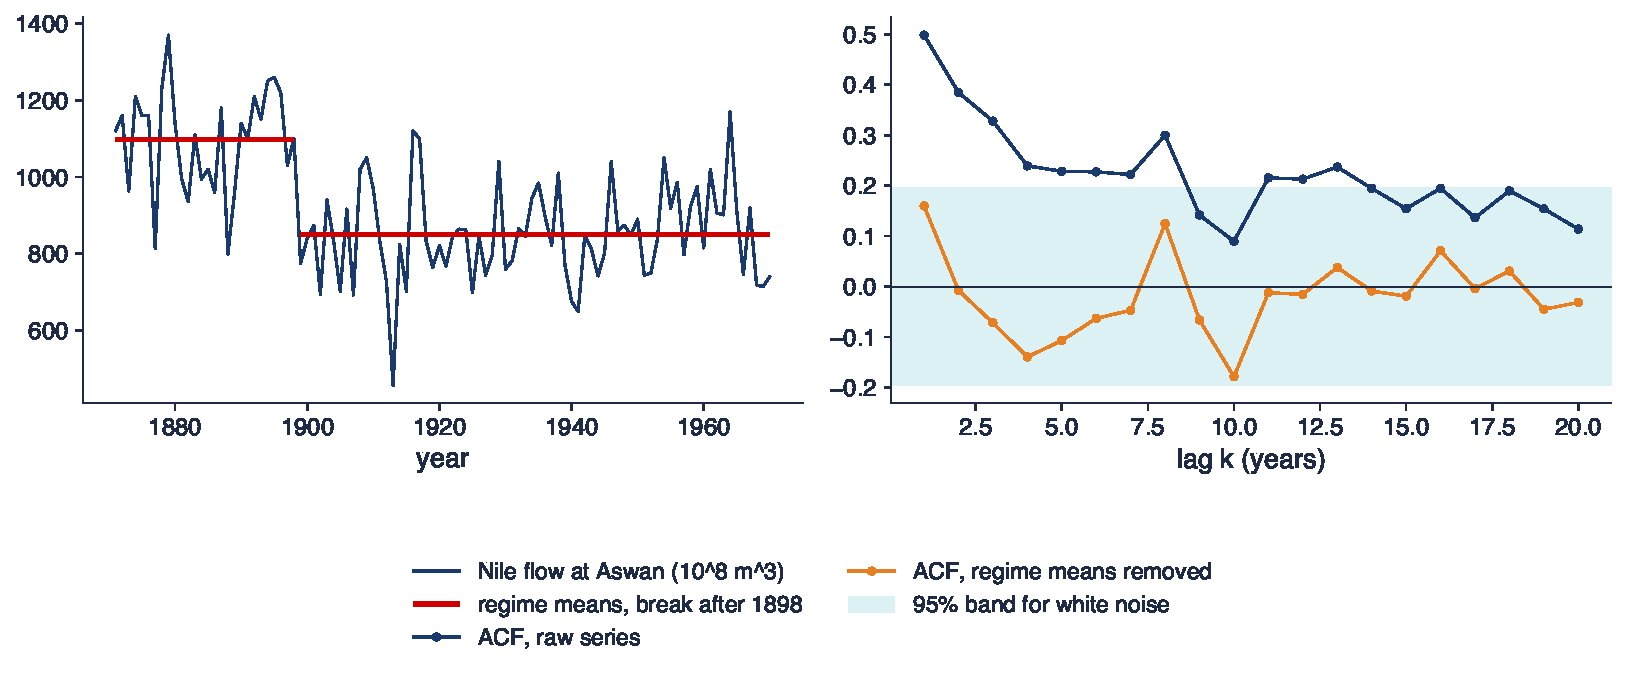
\includegraphics[width=0.96\textwidth,height=0.42\textheight,keepaspectratio]{ch8_sem_b1.pdf}
\end{center}
\vspace{-2mm}
\begin{itemize}
    \item Seria brută: $\hat\rho(1) = 0{,}50$, $\hat\rho(10) = 0{,}09$; $H_{R/S} = 0{,}78$; GPH 0{,}44 (SE 0{,}15), LW 0{,}40 (SE 0{,}11), ML 0{,}36 (SE 0{,}07); $m = 19$
    \item Mediile 1098 și 850; după eliminarea lor: $\hat\rho(1) = 0{,}16$; $H_{R/S} = 0{,}63$; GPH -0{,}07, LW -0{,}17, ML 0{,}05 (SE 0{,}10)
    \item Interpretare: pentru 1871--1970 dovada de memorie lungă provine dintr-o singură ruptură; R/S rămîne peste 0,5 deoarece este deplasat în sus în eșantioane scurte
\end{itemize}\quantlet{TSA\_ch8\_seminar}{\qlurl{TSA_ch8_seminar}}
\end{frame}

\begin{frame}{B2: memoria lungă a inflației din România [Propus]}
\itemsize{\footnotesize}
\begin{itemize}
\item \textbf{Întrebarea}: cît de persistentă este inflația din România și schimbă modul de măsurare a inflației răspunsul?
\item \textbf{Date}: IAPC lunar, 2005--2026: rata lunară ajustată sezonier cu mediile lunare și rata anuală; model: B1
\item \textbf{Cerințe}
\begin{enumerate}
    \item Estimați $d$ al ratei lunare prin GPH și Whittle local, cu $m = \lfloor T^a\rfloor$, $a = 0{,}5;\ 0{,}65;\ 0{,}8$.
    \item Estimați ARFIMA$(0,d,0)$ și ARMA(1,1) prin ML exactă și comparați BIC.
    \item Estimați $d$ al ratei anuale prin Whittle local și comparați cele două ACF.
    \item Interpretare: de ce dă rata anuală un $d$ apropiat de 1?
\end{enumerate}
\item \textbf{Raportați}: șase estimări, două valori BIC, un $d$, două fraze
\item Notebook: secțiunea B2
\end{itemize}
\end{frame}

\ifsolutions
\begin{frame}{B2: rezolvare [Propus]}
\itemsize{\scriptsize}
\begin{center}
\includegraphics[width=0.96\textwidth,height=0.42\textheight,keepaspectratio]{ch8_sem_b2.pdf}
\end{center}
\vspace{-2mm}
\begin{itemize}
    \item $T = 260$; GPH / LW: 0{,}56 / 0{,}58 ($m = 16$), 0{,}37 / 0{,}31 ($m = 37$), 0{,}62 / 0{,}29 ($m = 85$)
    \item ML exactă: $\hat d = 0{,}31$ (SE 0{,}047), BIC 282{,}9; ARMA(1,1): $\phi = 0{,}92$, $\theta = -0{,}71$, BIC 292{,}8: preferăm ARFIMA
    \item Rata anuală: LW 1{,}00, GPH 1{,}14; $\hat\rho(1)$ 0{,}98, față de 0{,}44 pentru rata lunară
    \item Interpretare: două rate anuale consecutive au 11 luni comune; suprapunerea este un filtru care elimină puterea la frecvențele din jurul lui $2\pi/12$ și înclină log-periodograma: $\hat d$ este împins spre 1
\end{itemize}\quantlet{TSA\_ch8\_seminar}{\qlurl{TSA_ch8_seminar}}
\end{frame}
\fi

\begin{frame}{B3: memoria volatilității S\&P 500 [Rezolvat]}
\itemsize{\footnotesize}
\begin{itemize}
\item \textbf{Întrebarea}: unde se află memoria randamentelor bursiere: în randamente sau în mărimea lor?
\item \textbf{Date}: randamentele logaritmice zilnice S\&P 500 din 2000 și volatilitatea lor realizată lunară
\item \textbf{Cerințe}
\begin{enumerate}
    \item Estimați $d$ pentru $r_t$ și pentru $|r_t|$ prin Whittle local și GPH.
    \item Permutați aleator zilele și reestimați $d$ pentru $|r_t|$; reprezentați grafic ambele ACF ale lui $|r_t|$.
    \item Estimați $d$ pentru logaritmul volatilității realizate lunare.
    \item Interpretare: ce arată testul permutării?
\end{enumerate}
\item \textbf{Raportați}: opt estimări, graficul și o frază
\item Notebook: secțiunea B3
\end{itemize}
\end{frame}

\begin{frame}{B3: rezolvare [Rezolvat]}
\itemsize{\scriptsize}
\begin{center}
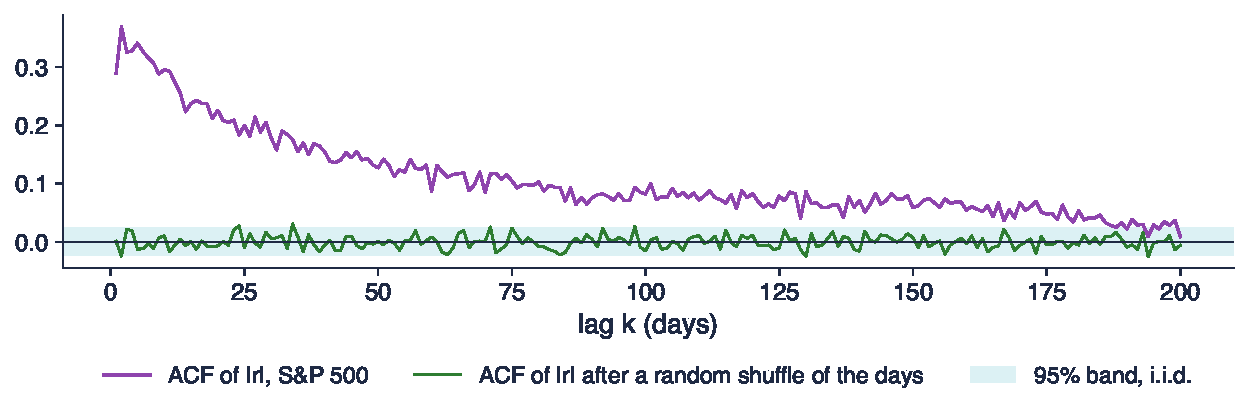
\includegraphics[width=0.96\textwidth,height=0.42\textheight,keepaspectratio]{ch8_sem_b3.pdf}
\end{center}
\vspace{-2mm}
\begin{itemize}
    \item $T = 6\,714$ de zile; $r_t$: LW -0{,}01, GPH 0{,}02 (SE 0{,}03; 0{,}04); $|r_t|$: LW 0{,}53, GPH 0{,}56
    \item $|r_t|$ permutat: LW -0{,}03, GPH -0{,}03; ACF a lui $|r_t|$: 0{,}289 (decalajul 1), 0{,}127 (decalajul 50), 0{,}009 (decalajul 200); log RV (321 de luni): LW 0{,}41, GPH 0{,}37
    \item Interpretare: permutarea păstrează fiecare valoare zilnică și le distruge ordinea; memoria dispare, deci ea se află în gruparea perioadelor calme și agitate, nu în distribuția randamentelor
\end{itemize}\quantlet{TSA\_ch8\_seminar}{\qlurl{TSA_ch8_seminar}}
\end{frame}

\begin{frame}{B4: BET și EUR/RON [Propus]}
\itemsize{\footnotesize}
\begin{itemize}
\item \textbf{Întrebarea}: au BET și cursul EUR/RON aceeași memorie și este ea stabilă înainte și după criza din 2008?
\item \textbf{Date}: randamentele logaritmice zilnice ale BET (din 2000) și ale cursului de referință EUR/RON (din iulie 2005); model: B3
\item \textbf{Cerințe}
\begin{enumerate}
    \item Estimați $d$ pentru $r_t$ și $|r_t|$ prin Whittle local pe tot eșantionul.
    \item Repetați pe subeșantioanele pînă în 2007 și 2010--2026.
    \item Comparați estimările pentru $r_t$ cu banda Monte Carlo de 95\% a seriilor i.i.d. de 1900 de zile.
    \item Interpretare: este reală memoria randamentelor BET pe tot eșantionul?
\end{enumerate}
\item \textbf{Raportați}: douăsprezece estimări, o bandă și două fraze
\item Notebook: secțiunea B4
\end{itemize}
\end{frame}

\ifsolutions
\begin{frame}{B4: rezolvare [Propus]}
\itemsize{\scriptsize}
\begin{center}
\includegraphics[width=0.96\textwidth,height=0.42\textheight,keepaspectratio]{ch8_sem_b4.pdf}
\end{center}
\vspace{-2mm}
\begin{itemize}
    \item BET $r_t$: 0{,}12 (tot), 0{,}01 (pînă în 2007), 0{,}02 (2010--2026); $|r_t|$: 0{,}39; 0{,}26; 0{,}39
    \item EUR/RON $r_t$: -0{,}01; -0{,}01; -0{,}05; $|r_t|$: 0{,}39; 0{,}18; 0{,}37; banda [-0{,}09; 0{,}10]
    \item Interpretare: memoria randamentelor BET pe tot eșantionul (0{,}12) dispare în fiecare subeșantion: provine din schimbarea de nivel și de volatilitate din jurul anului 2008, o memorie lungă aparentă; memoria lui $|r_t|$ rezistă pe ambele piețe
\end{itemize}\quantlet{TSA\_ch8\_seminar}{\qlurl{TSA_ch8_seminar}}
\end{frame}
\fi


%=============================================================================
\section{Partea C: întrebări deschise și critica unui răspuns AI}
%=============================================================================

\begin{frame}{C1: inflația din SUA și regimurile monetare [Propus]}
\itemsize{\footnotesize}
\begin{itemize}
\item \textbf{Întrebarea}: este memoria lungă a inflației din SUA o proprietate a inflației sau a schimbărilor de politică monetară?
\item \textbf{Date}: inflația lunară IPC din SUA, anualizată, 1947--2026; regimurile 1947--1984, 1985--2019, 2020--2026; modele: B1, B2
\item \textbf{Cerințe}
\begin{enumerate}
    \item Estimați $d$ prin Whittle local pe tot eșantionul și în fiecare regim.
    \item Eliminați cele trei medii de regim și reestimați $d$.
    \item Propuneți încă o verificare (un test de ruptură, un model Markov switching, o comparație de prognoze).
    \item Interpretare: poate un $d$ constant să descrie 80 de ani de inflație?
\end{enumerate}
\item \textbf{Raportați}: cinci estimări, o verificare și un plan de proiect
\item Notebook: secțiunea C1
\end{itemize}
\end{frame}

\ifsolutions
\begin{frame}{C1: analiză de referință [Propus]}
\itemsize{\scriptsize}
\begin{center}
\includegraphics[width=0.96\textwidth,height=0.42\textheight,keepaspectratio]{ch8_sem_c1.pdf}
\end{center}
\vspace{-2mm}
\begin{itemize}
    \item $\hat d$: tot eșantionul 0{,}55; 1947--1984 0{,}48 (media 4{,}20\%); 1985--2019 0{,}10 (media 2{,}56\%); 2020--2026 0{,}27 (79 de luni)
    \item Fără mediile de regim: 0{,}53: schimbările de medie singure nu elimină memoria; ea se află în interiorul regimului 1947--1984 (Marea Inflație)
    \item Interpretare: nu; memoria este puternică atunci cînd politica lasă inflația să derive și slabă sub țintirea inflației; $d$ este o proprietate a regimului de politică, o legătură naturală cu \tsachlink{https://danpele.github.io/Time-Series-Analysis/RO/Cursuri/capitol10_spatiul_starilor_kalman_markov_switching.pdf}{Capitolul 10}
    \item Proiect: aceeași analiză pentru România (IAPC lunar din 1997), cu trecerea la țintirea inflației din 2005
\end{itemize}\quantlet{TSA\_ch8\_seminar}{\qlurl{TSA_ch8_seminar}}
\end{frame}
\fi

\begin{frame}{C2: verificați un răspuns AI [Propus]}
\itemsize{\scriptsize}
\begin{itemize}
    \item Un student a întrebat un asistent AI despre memoria lungă a inflației din România și a S\&P 500. Răspunsul:
    \item \aiprompt{(a) Inflația lunară are d = 0{,}31, deci exponentul Hurst este H = d - 0,5 < 0: este antipersistentă.}
    \item \aiprompt{(b) Rata anuală dă d = 1{,}00, deci inflația din România are rădăcină unitară.}
    \item \aiprompt{(c) Cu d = 0{,}31 seria este staționară, iar șocurile ei se sting.}
    \item \aiprompt{(d) Folosiți statsmodels.tsa.arima.model.ARIMA(x, order=(0, 0.31, 0)) pentru a estima modelul ARFIMA.}
    \item \aiprompt{(e) Randamentele S\&P 500 au d = -0{,}01, iar |r| are d = 0{,}53, deci randamentele sînt previzibile.}
    \item \aiprompt{(f) O estimare GPH semnificativă demonstrează memoria lungă.}
    \item Cerințe
    \begin{itemize}
        \item 1. Pentru fiecare afirmație, precizați dacă este corectă; dacă nu este, formulați afirmația corectă și, acolo unde se poate, dați valoarea corectă din notebook (secțiunea C2).
        \item 2. Raportați: o listă de șase verdicte, fiecare cu un rînd de justificare.
    \end{itemize}
\end{itemize}
\end{frame}

\ifsolutions
\begin{frame}{C2: rezolvare [Propus]}
\itemsize{\scriptsize}
\begin{itemize}
    \item (a) Greșit: $H = d + 0{,}5 = 0{,}81$: persistentă
    \item (b) Greșit: suprapunerea ratelor anuale împinge $\hat d$ spre 1 (B2); rata lunară dă $d = 0{,}31$
    \item (c) Corect: $0 < d < 0{,}5$; șocurile se sting hiperbolic, mai lent decît în ARMA
    \item (d) Greșit: ordinul ARIMA trebuie să fie întreg; statsmodels nu are o clasă ARFIMA (folosiți ML exactă sau Whittle, ca în notebook)
    \item (e) Greșit: $d \approx 0$ pentru randamente înseamnă că randamentele nu au memorie; memoria lui $|r_t|$ face volatilitatea previzibilă, nu semnul
    \item (f) Greșit: rupturile și schimbările de regim dau și ele un $\hat d$ semnificativ (B1, B4)
\end{itemize}\quantlet{TSA\_ch8\_seminar}{\qlurl{TSA_ch8_seminar}}
\end{frame}
\fi


%=============================================================================
\section{Încheiere}
%=============================================================================

\begin{frame}{Idei de reținut}
\itemsize{\small}
\begin{itemize}
    \item $(1-L)^d$: ponderile prin recurența $\pi_k = \pi_{k-1}(k-1-d)/k$; ARFIMA$(0,d,0)$: $\rho(1) = d/(1-d)$
    \item $H = d + 1/2$; R/S și GPH sînt pante ale unor regresii log--log
    \item Inflația lunară din România: $d \approx 0{,}3$; S\&P 500: memorie în $|r_t|$, nu în $r_t$
    \item Rupturile pot crea memorie lungă: Nilul, randamentele BET, inflația din SUA
    \item Un răspuns AI este o ciornă: verificați relația dintre $H$ și $d$, biblioteca și transformarea datelor
\end{itemize}
\end{frame}

\begin{frame}{După seminar}
\itemsize{\small}
\begin{itemize}
    \item Cursul 8 dezvoltă fiecare temă de azi: descreșterea hiperbolică, diferențierea fracționară, ARFIMA, estimatorii, prognoza, volatilitatea, memoria aparentă
    \item Încercați cerințele [Propus] în notebook
    \item C1 poate deveni un proiect de echipă: memoria inflației și regimurile monetare din România
    \item Lectură: \refBaillie; \refGraves; \refDGE
    \item \textbf{Seminarul are rol de exercițiu și nu se notează; rezolvările cerințelor [Propus] se discută la seminar}
\end{itemize}
\end{frame}


%=============================================================================
\section{Bibliografie}
%=============================================================================

\begin{frame}{Bibliografie}
\itemsize{\tiny}
\begin{itemize}
    \item Baillie, R. T. (1996). Long memory processes and fractional integration in econometrics. \textit{Journal of Econometrics}, 73(1), 5--59. \href{https://doi.org/10.1016/0304-4076(95)01732-1}{doi:10.1016/0304-4076(95)01732-1}
    \item Baillie, R. T., Bollerslev, T., \& Mikkelsen, H. O. (1996). Fractionally integrated generalized autoregressive conditional heteroskedasticity. \textit{Journal of Econometrics}, 74(1), 3--30. \href{https://doi.org/10.1016/S0304-4076(95)01749-6}{doi:10.1016/S0304-4076(95)01749-6}
    \item Diebold, F. X., \& Inoue, A. (2001). Long memory and regime switching. \textit{Journal of Econometrics}, 105(1), 131--159. \href{https://doi.org/10.1016/S0304-4076(01)00073-2}{doi:10.1016/S0304-4076(01)00073-2}
    \item Ding, Z., Granger, C. W. J., \& Engle, R. F. (1993). A long memory property of stock market returns and a new model. \textit{Journal of Empirical Finance}, 1(1), 83--106. \href{https://doi.org/10.1016/0927-5398(93)90006-D}{doi:10.1016/0927-5398(93)90006-D}
    \item Granger, C. W. J., \& Joyeux, R. (1980). An introduction to long-memory time series models and fractional differencing. \textit{Journal of Time Series Analysis}, 1(1), 15--29. \href{https://doi.org/10.1111/j.1467-9892.1980.tb00297.x}{doi:10.1111/j.1467-9892.1980.tb00297.x}
    \item Graves, T., Gramacy, R., Watkins, N., \& Franzke, C. (2017). A brief history of long memory: Hurst, Mandelbrot and the road to ARFIMA, 1951--1980. \textit{Entropy}, 19(9), 437. \href{https://doi.org/10.3390/e19090437}{doi:10.3390/e19090437}
    \item Hosking, J. R. M. (1981). Fractional differencing. \textit{Biometrika}, 68(1), 165--176. \href{https://doi.org/10.1093/biomet/68.1.165}{doi:10.1093/biomet/68.1.165}
    \item Hurst, H. E. (1951). Long-term storage capacity of reservoirs. \textit{Transactions of the American Society of Civil Engineers}, 116(1), 770--799. \href{https://doi.org/10.1061/TACEAT.0006518}{doi:10.1061/TACEAT.0006518}
    \item Robinson, P. M. (1995). Gaussian semiparametric estimation of long range dependence. \textit{The Annals of Statistics}, 23(5), 1630--1661. \href{https://doi.org/10.1214/aos/1176324317}{doi:10.1214/aos/1176324317}
    \item Sowell, F. (1992). Maximum likelihood estimation of stationary univariate fractionally integrated time series models. \textit{Journal of Econometrics}, 53(1--3), 165--188. \href{https://doi.org/10.1016/0304-4076(92)90084-5}{doi:10.1016/0304-4076(92)90084-5}
\end{itemize}
\end{frame}

\end{document}
